% GNU GENERAL PUBLIC LICENSE
%                        Version 3, 29 June 2007

%  Copyright (C) 2007 Free Software Foundation, Inc. <https://fsf.org/>
%  Everyone is permitted to copy and distribute verbatim copies
%  of this license document, but changing it is not allowed.

%                             Preamble

%   The GNU General Public License is a free, copyleft license for
% software and other kinds of works.

%   The licenses for most software and other practical works are designed
% to take away your freedom to share and change the works.  By contrast,
% the GNU General Public License is intended to guarantee your freedom to
% share and change all versions of a program--to make sure it remains free
% software for all its users.  We, the Free Software Foundation, use the
% GNU General Public License for most of our software; it applies also to
% any other work released this way by its authors.  You can apply it to
% your programs, too.

%   When we speak of free software, we are referring to freedom, not
% price.  Our General Public Licenses are designed to make sure that you
% have the freedom to distribute copies of free software (and charge for
% them if you wish), that you receive source code or can get it if you
% want it, that you can change the software or use pieces of it in new
% free programs, and that you know you can do these things.

%   To protect your rights, we need to prevent others from denying you
% these rights or asking you to surrender the rights.  Therefore, you have
% certain responsibilities if you distribute copies of the software, or if
% you modify it: responsibilities to respect the freedom of others.

%   For example, if you distribute copies of such a program, whether
% gratis or for a fee, you must pass on to the recipients the same
% freedoms that you received.  You must make sure that they, too, receive
% or can get the source code.  And you must show them these terms so they
% know their rights.

%   Developers that use the GNU GPL protect your rights with two steps:
% (1) assert copyright on the software, and (2) offer you this License
% giving you legal permission to copy, distribute and/or modify it.

%   For the developers' and authors' protection, the GPL clearly explains
% that there is no warranty for this free software.  For both users' and
% authors' sake, the GPL requires that modified versions be marked as
% changed, so that their problems will not be attributed erroneously to
% authors of previous versions.

%   Some devices are designed to deny users access to install or run
% modified versions of the software inside them, although the manufacturer
% can do so.  This is fundamentally incompatible with the aim of
% protecting users' freedom to change the software.  The systematic
% pattern of such abuse occurs in the area of products for individuals to
% use, which is precisely where it is most unacceptable.  Therefore, we
% have designed this version of the GPL to prohibit the practice for those
% products.  If such problems arise substantially in other domains, we
% stand ready to extend this provision to those domains in future versions
% of the GPL, as needed to protect the freedom of users.

%   Finally, every program is threatened constantly by software patents.
% States should not allow patents to restrict development and use of
% software on general-purpose computers, but in those that do, we wish to
% avoid the special danger that patents applied to a free program could
% make it effectively proprietary.  To prevent this, the GPL assures that
% patents cannot be used to render the program non-free.

%   The precise terms and conditions for copying, distribution and
% modification follow.

%                        TERMS AND CONDITIONS

%   0. Definitions.

%   "This License" refers to version 3 of the GNU General Public License.

%   "Copyright" also means copyright-like laws that apply to other kinds of
% works, such as semiconductor masks.

%   "The Program" refers to any copyrightable work licensed under this
% License.  Each licensee is addressed as "you".  "Licensees" and
% "recipients" may be individuals or organizations.

%   To "modify" a work means to copy from or adapt all or part of the work
% in a fashion requiring copyright permission, other than the making of an
% exact copy.  The resulting work is called a "modified version" of the
% earlier work or a work "based on" the earlier work.

%   A "covered work" means either the unmodified Program or a work based
% on the Program.

%   To "propagate" a work means to do anything with it that, without
% permission, would make you directly or secondarily liable for
% infringement under applicable copyright law, except executing it on a
% computer or modifying a private copy.  Propagation includes copying,
% distribution (with or without modification), making available to the
% public, and in some countries other activities as well.

%   To "convey" a work means any kind of propagation that enables other
% parties to make or receive copies.  Mere interaction with a user through
% a computer network, with no transfer of a copy, is not conveying.

%   An interactive user interface displays "Appropriate Legal Notices"
% to the extent that it includes a convenient and prominently visible
% feature that (1) displays an appropriate copyright notice, and (2)
% tells the user that there is no warranty for the work (except to the
% extent that warranties are provided), that licensees may convey the
% work under this License, and how to view a copy of this License.  If
% the interface presents a list of user commands or options, such as a
% menu, a prominent item in the list meets this criterion.

%   1. Source Code.

%   The "source code" for a work means the preferred form of the work
% for making modifications to it.  "Object code" means any non-source
% form of a work.

%   A "Standard Interface" means an interface that either is an official
% standard defined by a recognized standards body, or, in the case of
% interfaces specified for a particular programming language, one that
% is widely used among developers working in that language.

%   The "System Libraries" of an executable work include anything, other
% than the work as a whole, that (a) is included in the normal form of
% packaging a Major Component, but which is not part of that Major
% Component, and (b) serves only to enable use of the work with that
% Major Component, or to implement a Standard Interface for which an
% implementation is available to the public in source code form.  A
% "Major Component", in this context, means a major essential component
% (kernel, window system, and so on) of the specific operating system
% (if any) on which the executable work runs, or a compiler used to
% produce the work, or an object code interpreter used to run it.

%   The "Corresponding Source" for a work in object code form means all
% the source code needed to generate, install, and (for an executable
% work) run the object code and to modify the work, including scripts to
% control those activities.  However, it does not include the work's
% System Libraries, or general-purpose tools or generally available free
% programs which are used unmodified in performing those activities but
% which are not part of the work.  For example, Corresponding Source
% includes interface definition files associated with source files for
% the work, and the source code for shared libraries and dynamically
% linked subprograms that the work is specifically designed to require,
% such as by intimate data communication or control flow between those
% subprograms and other parts of the work.

%   The Corresponding Source need not include anything that users
% can regenerate automatically from other parts of the Corresponding
% Source.

%   The Corresponding Source for a work in source code form is that
% same work.

%   2. Basic Permissions.

%   All rights granted under this License are granted for the term of
% copyright on the Program, and are irrevocable provided the stated
% conditions are met.  This License explicitly affirms your unlimited
% permission to run the unmodified Program.  The output from running a
% covered work is covered by this License only if the output, given its
% content, constitutes a covered work.  This License acknowledges your
% rights of fair use or other equivalent, as provided by copyright law.

%   You may make, run and propagate covered works that you do not
% convey, without conditions so long as your license otherwise remains
% in force.  You may convey covered works to others for the sole purpose
% of having them make modifications exclusively for you, or provide you
% with facilities for running those works, provided that you comply with
% the terms of this License in conveying all material for which you do
% not control copyright.  Those thus making or running the covered works
% for you must do so exclusively on your behalf, under your direction
% and control, on terms that prohibit them from making any copies of
% your copyrighted material outside their relationship with you.

%   Conveying under any other circumstances is permitted solely under
% the conditions stated below.  Sublicensing is not allowed; section 10
% makes it unnecessary.

%   3. Protecting Users' Legal Rights From Anti-Circumvention Law.

%   No covered work shall be deemed part of an effective technological
% measure under any applicable law fulfilling obligations under article
% 11 of the WIPO copyright treaty adopted on 20 December 1996, or
% similar laws prohibiting or restricting circumvention of such
% measures.

%   When you convey a covered work, you waive any legal power to forbid
% circumvention of technological measures to the extent such circumvention
% is effected by exercising rights under this License with respect to
% the covered work, and you disclaim any intention to limit operation or
% modification of the work as a means of enforcing, against the work's
% users, your or third parties' legal rights to forbid circumvention of
% technological measures.

%   4. Conveying Verbatim Copies.

%   You may convey verbatim copies of the Program's source code as you
% receive it, in any medium, provided that you conspicuously and
% appropriately publish on each copy an appropriate copyright notice;
% keep intact all notices stating that this License and any
% non-permissive terms added in accord with section 7 apply to the code;
% keep intact all notices of the absence of any warranty; and give all
% recipients a copy of this License along with the Program.

%   You may charge any price or no price for each copy that you convey,
% and you may offer support or warranty protection for a fee.

%   5. Conveying Modified Source Versions.

%   You may convey a work based on the Program, or the modifications to
% produce it from the Program, in the form of source code under the
% terms of section 4, provided that you also meet all of these conditions:

%     a) The work must carry prominent notices stating that you modified
%     it, and giving a relevant date.

%     b) The work must carry prominent notices stating that it is
%     released under this License and any conditions added under section
%     7.  This requirement modifies the requirement in section 4 to
%     "keep intact all notices".

%     c) You must license the entire work, as a whole, under this
%     License to anyone who comes into possession of a copy.  This
%     License will therefore apply, along with any applicable section 7
%     additional terms, to the whole of the work, and all its parts,
%     regardless of how they are packaged.  This License gives no
%     permission to license the work in any other way, but it does not
%     invalidate such permission if you have separately received it.

%     d) If the work has interactive user interfaces, each must display
%     Appropriate Legal Notices; however, if the Program has interactive
%     interfaces that do not display Appropriate Legal Notices, your
%     work need not make them do so.

%   A compilation of a covered work with other separate and independent
% works, which are not by their nature extensions of the covered work,
% and which are not combined with it such as to form a larger program,
% in or on a volume of a storage or distribution medium, is called an
% "aggregate" if the compilation and its resulting copyright are not
% used to limit the access or legal rights of the compilation's users
% beyond what the individual works permit.  Inclusion of a covered work
% in an aggregate does not cause this License to apply to the other
% parts of the aggregate.

%   6. Conveying Non-Source Forms.

%   You may convey a covered work in object code form under the terms
% of sections 4 and 5, provided that you also convey the
% machine-readable Corresponding Source under the terms of this License,
% in one of these ways:

%     a) Convey the object code in, or embodied in, a physical product
%     (including a physical distribution medium), accompanied by the
%     Corresponding Source fixed on a durable physical medium
%     customarily used for software interchange.

%     b) Convey the object code in, or embodied in, a physical product
%     (including a physical distribution medium), accompanied by a
%     written offer, valid for at least three years and valid for as
%     long as you offer spare parts or customer support for that product
%     model, to give anyone who possesses the object code either (1) a
%     copy of the Corresponding Source for all the software in the
%     product that is covered by this License, on a durable physical
%     medium customarily used for software interchange, for a price no
%     more than your reasonable cost of physically performing this
%     conveying of source, or (2) access to copy the
%     Corresponding Source from a network server at no charge.

%     c) Convey individual copies of the object code with a copy of the
%     written offer to provide the Corresponding Source.  This
%     alternative is allowed only occasionally and noncommercially, and
%     only if you received the object code with such an offer, in accord
%     with subsection 6b.

%     d) Convey the object code by offering access from a designated
%     place (gratis or for a charge), and offer equivalent access to the
%     Corresponding Source in the same way through the same place at no
%     further charge.  You need not require recipients to copy the
%     Corresponding Source along with the object code.  If the place to
%     copy the object code is a network server, the Corresponding Source
%     may be on a different server (operated by you or a third party)
%     that supports equivalent copying facilities, provided you maintain
%     clear directions next to the object code saying where to find the
%     Corresponding Source.  Regardless of what server hosts the
%     Corresponding Source, you remain obligated to ensure that it is
%     available for as long as needed to satisfy these requirements.

%     e) Convey the object code using peer-to-peer transmission, provided
%     you inform other peers where the object code and Corresponding
%     Source of the work are being offered to the general public at no
%     charge under subsection 6d.

%   A separable portion of the object code, whose source code is excluded
% from the Corresponding Source as a System Library, need not be
% included in conveying the object code work.

%   A "User Product" is either (1) a "consumer product", which means any
% tangible personal property which is normally used for personal, family,
% or household purposes, or (2) anything designed or sold for incorporation
% into a dwelling.  In determining whether a product is a consumer product,
% doubtful cases shall be resolved in favor of coverage.  For a particular
% product received by a particular user, "normally used" refers to a
% typical or common use of that class of product, regardless of the status
% of the particular user or of the way in which the particular user
% actually uses, or expects or is expected to use, the product.  A product
% is a consumer product regardless of whether the product has substantial
% commercial, industrial or non-consumer uses, unless such uses represent
% the only significant mode of use of the product.

%   "Installation Information" for a User Product means any methods,
% procedures, authorization keys, or other information required to install
% and execute modified versions of a covered work in that User Product from
% a modified version of its Corresponding Source.  The information must
% suffice to ensure that the continued functioning of the modified object
% code is in no case prevented or interfered with solely because
% modification has been made.

%   If you convey an object code work under this section in, or with, or
% specifically for use in, a User Product, and the conveying occurs as
% part of a transaction in which the right of possession and use of the
% User Product is transferred to the recipient in perpetuity or for a
% fixed term (regardless of how the transaction is characterized), the
% Corresponding Source conveyed under this section must be accompanied
% by the Installation Information.  But this requirement does not apply
% if neither you nor any third party retains the ability to install
% modified object code on the User Product (for example, the work has
% been installed in ROM).

%   The requirement to provide Installation Information does not include a
% requirement to continue to provide support service, warranty, or updates
% for a work that has been modified or installed by the recipient, or for
% the User Product in which it has been modified or installed.  Access to a
% network may be denied when the modification itself materially and
% adversely affects the operation of the network or violates the rules and
% protocols for communication across the network.

%   Corresponding Source conveyed, and Installation Information provided,
% in accord with this section must be in a format that is publicly
% documented (and with an implementation available to the public in
% source code form), and must require no special password or key for
% unpacking, reading or copying.

%   7. Additional Terms.

%   "Additional permissions" are terms that supplement the terms of this
% License by making exceptions from one or more of its conditions.
% Additional permissions that are applicable to the entire Program shall
% be treated as though they were included in this License, to the extent
% that they are valid under applicable law.  If additional permissions
% apply only to part of the Program, that part may be used separately
% under those permissions, but the entire Program remains governed by
% this License without regard to the additional permissions.

%   When you convey a copy of a covered work, you may at your option
% remove any additional permissions from that copy, or from any part of
% it.  (Additional permissions may be written to require their own
% removal in certain cases when you modify the work.)  You may place
% additional permissions on material, added by you to a covered work,
% for which you have or can give appropriate copyright permission.

%   Notwithstanding any other provision of this License, for material you
% add to a covered work, you may (if authorized by the copyright holders of
% that material) supplement the terms of this License with terms:

%     a) Disclaiming warranty or limiting liability differently from the
%     terms of sections 15 and 16 of this License; or

%     b) Requiring preservation of specified reasonable legal notices or
%     author attributions in that material or in the Appropriate Legal
%     Notices displayed by works containing it; or

%     c) Prohibiting misrepresentation of the origin of that material, or
%     requiring that modified versions of such material be marked in
%     reasonable ways as different from the original version; or

%     d) Limiting the use for publicity purposes of names of licensors or
%     authors of the material; or

%     e) Declining to grant rights under trademark law for use of some
%     trade names, trademarks, or service marks; or

%     f) Requiring indemnification of licensors and authors of that
%     material by anyone who conveys the material (or modified versions of
%     it) with contractual assumptions of liability to the recipient, for
%     any liability that these contractual assumptions directly impose on
%     those licensors and authors.

%   All other non-permissive additional terms are considered "further
% restrictions" within the meaning of section 10.  If the Program as you
% received it, or any part of it, contains a notice stating that it is
% governed by this License along with a term that is a further
% restriction, you may remove that term.  If a license document contains
% a further restriction but permits relicensing or conveying under this
% License, you may add to a covered work material governed by the terms
% of that license document, provided that the further restriction does
% not survive such relicensing or conveying.

%   If you add terms to a covered work in accord with this section, you
% must place, in the relevant source files, a statement of the
% additional terms that apply to those files, or a notice indicating
% where to find the applicable terms.

%   Additional terms, permissive or non-permissive, may be stated in the
% form of a separately written license, or stated as exceptions;
% the above requirements apply either way.

%   8. Termination.

%   You may not propagate or modify a covered work except as expressly
% provided under this License.  Any attempt otherwise to propagate or
% modify it is void, and will automatically terminate your rights under
% this License (including any patent licenses granted under the third
% paragraph of section 11).

%   However, if you cease all violation of this License, then your
% license from a particular copyright holder is reinstated (a)
% provisionally, unless and until the copyright holder explicitly and
% finally terminates your license, and (b) permanently, if the copyright
% holder fails to notify you of the violation by some reasonable means
% prior to 60 days after the cessation.

%   Moreover, your license from a particular copyright holder is
% reinstated permanently if the copyright holder notifies you of the
% violation by some reasonable means, this is the first time you have
% received notice of violation of this License (for any work) from that
% copyright holder, and you cure the violation prior to 30 days after
% your receipt of the notice.

%   Termination of your rights under this section does not terminate the
% licenses of parties who have received copies or rights from you under
% this License.  If your rights have been terminated and not permanently
% reinstated, you do not qualify to receive new licenses for the same
% material under section 10.

%   9. Acceptance Not Required for Having Copies.

%   You are not required to accept this License in order to receive or
% run a copy of the Program.  Ancillary propagation of a covered work
% occurring solely as a consequence of using peer-to-peer transmission
% to receive a copy likewise does not require acceptance.  However,
% nothing other than this License grants you permission to propagate or
% modify any covered work.  These actions infringe copyright if you do
% not accept this License.  Therefore, by modifying or propagating a
% covered work, you indicate your acceptance of this License to do so.

%   10. Automatic Licensing of Downstream Recipients.

%   Each time you convey a covered work, the recipient automatically
% receives a license from the original licensors, to run, modify and
% propagate that work, subject to this License.  You are not responsible
% for enforcing compliance by third parties with this License.

%   An "entity transaction" is a transaction transferring control of an
% organization, or substantially all assets of one, or subdividing an
% organization, or merging organizations.  If propagation of a covered
% work results from an entity transaction, each party to that
% transaction who receives a copy of the work also receives whatever
% licenses to the work the party's predecessor in interest had or could
% give under the previous paragraph, plus a right to possession of the
% Corresponding Source of the work from the predecessor in interest, if
% the predecessor has it or can get it with reasonable efforts.

%   You may not impose any further restrictions on the exercise of the
% rights granted or affirmed under this License.  For example, you may
% not impose a license fee, royalty, or other charge for exercise of
% rights granted under this License, and you may not initiate litigation
% (including a cross-claim or counterclaim in a lawsuit) alleging that
% any patent claim is infringed by making, using, selling, offering for
% sale, or importing the Program or any portion of it.

%   11. Patents.

%   A "contributor" is a copyright holder who authorizes use under this
% License of the Program or a work on which the Program is based.  The
% work thus licensed is called the contributor's "contributor version".

%   A contributor's "essential patent claims" are all patent claims
% owned or controlled by the contributor, whether already acquired or
% hereafter acquired, that would be infringed by some manner, permitted
% by this License, of making, using, or selling its contributor version,
% but do not include claims that would be infringed only as a
% consequence of further modification of the contributor version.  For
% purposes of this definition, "control" includes the right to grant
% patent sublicenses in a manner consistent with the requirements of
% this License.

%   Each contributor grants you a non-exclusive, worldwide, royalty-free
% patent license under the contributor's essential patent claims, to
% make, use, sell, offer for sale, import and otherwise run, modify and
% propagate the contents of its contributor version.

%   In the following three paragraphs, a "patent license" is any express
% agreement or commitment, however denominated, not to enforce a patent
% (such as an express permission to practice a patent or covenant not to
% sue for patent infringement).  To "grant" such a patent license to a
% party means to make such an agreement or commitment not to enforce a
% patent against the party.

%   If you convey a covered work, knowingly relying on a patent license,
% and the Corresponding Source of the work is not available for anyone
% to copy, free of charge and under the terms of this License, through a
% publicly available network server or other readily accessible means,
% then you must either (1) cause the Corresponding Source to be so
% available, or (2) arrange to deprive yourself of the benefit of the
% patent license for this particular work, or (3) arrange, in a manner
% consistent with the requirements of this License, to extend the patent
% license to downstream recipients.  "Knowingly relying" means you have
% actual knowledge that, but for the patent license, your conveying the
% covered work in a country, or your recipient's use of the covered work
% in a country, would infringe one or more identifiable patents in that
% country that you have reason to believe are valid.

%   If, pursuant to or in connection with a single transaction or
% arrangement, you convey, or propagate by procuring conveyance of, a
% covered work, and grant a patent license to some of the parties
% receiving the covered work authorizing them to use, propagate, modify
% or convey a specific copy of the covered work, then the patent license
% you grant is automatically extended to all recipients of the covered
% work and works based on it.

%   A patent license is "discriminatory" if it does not include within
% the scope of its coverage, prohibits the exercise of, or is
% conditioned on the non-exercise of one or more of the rights that are
% specifically granted under this License.  You may not convey a covered
% work if you are a party to an arrangement with a third party that is
% in the business of distributing software, under which you make payment
% to the third party based on the extent of your activity of conveying
% the work, and under which the third party grants, to any of the
% parties who would receive the covered work from you, a discriminatory
% patent license (a) in connection with copies of the covered work
% conveyed by you (or copies made from those copies), or (b) primarily
% for and in connection with specific products or compilations that
% contain the covered work, unless you entered into that arrangement,
% or that patent license was granted, prior to 28 March 2007.

%   Nothing in this License shall be construed as excluding or limiting
% any implied license or other defenses to infringement that may
% otherwise be available to you under applicable patent law.

%   12. No Surrender of Others' Freedom.

%   If conditions are imposed on you (whether by court order, agreement or
% otherwise) that contradict the conditions of this License, they do not
% excuse you from the conditions of this License.  If you cannot convey a
% covered work so as to satisfy simultaneously your obligations under this
% License and any other pertinent obligations, then as a consequence you may
% not convey it at all.  For example, if you agree to terms that obligate you
% to collect a royalty for further conveying from those to whom you convey
% the Program, the only way you could satisfy both those terms and this
% License would be to refrain entirely from conveying the Program.

%   13. Use with the GNU Affero General Public License.

%   Notwithstanding any other provision of this License, you have
% permission to link or combine any covered work with a work licensed
% under version 3 of the GNU Affero General Public License into a single
% combined work, and to convey the resulting work.  The terms of this
% License will continue to apply to the part which is the covered work,
% but the special requirements of the GNU Affero General Public License,
% section 13, concerning interaction through a network will apply to the
% combination as such.

%   14. Revised Versions of this License.

%   The Free Software Foundation may publish revised and/or new versions of
% the GNU General Public License from time to time.  Such new versions will
% be similar in spirit to the present version, but may differ in detail to
% address new problems or concerns.

%   Each version is given a distinguishing version number.  If the
% Program specifies that a certain numbered version of the GNU General
% Public License "or any later version" applies to it, you have the
% option of following the terms and conditions either of that numbered
% version or of any later version published by the Free Software
% Foundation.  If the Program does not specify a version number of the
% GNU General Public License, you may choose any version ever published
% by the Free Software Foundation.

%   If the Program specifies that a proxy can decide which future
% versions of the GNU General Public License can be used, that proxy's
% public statement of acceptance of a version permanently authorizes you
% to choose that version for the Program.

%   Later license versions may give you additional or different
% permissions.  However, no additional obligations are imposed on any
% author or copyright holder as a result of your choosing to follow a
% later version.

%   15. Disclaimer of Warranty.

%   THERE IS NO WARRANTY FOR THE PROGRAM, TO THE EXTENT PERMITTED BY
% APPLICABLE LAW.  EXCEPT WHEN OTHERWISE STATED IN WRITING THE COPYRIGHT
% HOLDERS AND/OR OTHER PARTIES PROVIDE THE PROGRAM "AS IS" WITHOUT WARRANTY
% OF ANY KIND, EITHER EXPRESSED OR IMPLIED, INCLUDING, BUT NOT LIMITED TO,
% THE IMPLIED WARRANTIES OF MERCHANTABILITY AND FITNESS FOR A PARTICULAR
% PURPOSE.  THE ENTIRE RISK AS TO THE QUALITY AND PERFORMANCE OF THE PROGRAM
% IS WITH YOU.  SHOULD THE PROGRAM PROVE DEFECTIVE, YOU ASSUME THE COST OF
% ALL NECESSARY SERVICING, REPAIR OR CORRECTION.

%   16. Limitation of Liability.

%   IN NO EVENT UNLESS REQUIRED BY APPLICABLE LAW OR AGREED TO IN WRITING
% WILL ANY COPYRIGHT HOLDER, OR ANY OTHER PARTY WHO MODIFIES AND/OR CONVEYS
% THE PROGRAM AS PERMITTED ABOVE, BE LIABLE TO YOU FOR DAMAGES, INCLUDING ANY
% GENERAL, SPECIAL, INCIDENTAL OR CONSEQUENTIAL DAMAGES ARISING OUT OF THE
% USE OR INABILITY TO USE THE PROGRAM (INCLUDING BUT NOT LIMITED TO LOSS OF
% DATA OR DATA BEING RENDERED INACCURATE OR LOSSES SUSTAINED BY YOU OR THIRD
% PARTIES OR A FAILURE OF THE PROGRAM TO OPERATE WITH ANY OTHER PROGRAMS),
% EVEN IF SUCH HOLDER OR OTHER PARTY HAS BEEN ADVISED OF THE POSSIBILITY OF
% SUCH DAMAGES.

%   17. Interpretation of Sections 15 and 16.

%   If the disclaimer of warranty and limitation of liability provided
% above cannot be given local legal effect according to their terms,
% reviewing courts shall apply local law that most closely approximates
% an absolute waiver of all civil liability in connection with the
% Program, unless a warranty or assumption of liability accompanies a
% copy of the Program in return for a fee.

%                      END OF TERMS AND CONDITIONS

%             How to Apply These Terms to Your New Programs

%   If you develop a new program, and you want it to be of the greatest
% possible use to the public, the best way to achieve this is to make it
% free software which everyone can redistribute and change under these terms.

%   To do so, attach the following notices to the program.  It is safest
% to attach them to the start of each source file to most effectively
% state the exclusion of warranty; and each file should have at least
% the "copyright" line and a pointer to where the full notice is found.

%     <one line to give the program's name and a brief idea of what it does.>
%     Copyright (C) <year>  <name of author>

%     This program is free software: you can redistribute it and/or modify
%     it under the terms of the GNU General Public License as published by
%     the Free Software Foundation, either version 3 of the License, or
%     (at your option) any later version.

%     This program is distributed in the hope that it will be useful,
%     but WITHOUT ANY WARRANTY; without even the implied warranty of
%     MERCHANTABILITY or FITNESS FOR A PARTICULAR PURPOSE.  See the
%     GNU General Public License for more details.

%     You should have received a copy of the GNU General Public License
%     along with this program.  If not, see <https://www.gnu.org/licenses/>.

% Also add information on how to contact you by electronic and paper mail.

%   If the program does terminal interaction, make it output a short
% notice like this when it starts in an interactive mode:

%     <program>  Copyright (C) <year>  <name of author>
%     This program comes with ABSOLUTELY NO WARRANTY; for details type `show w'.
%     This is free software, and you are welcome to redistribute it
%     under certain conditions; type `show c' for details.

% The hypothetical commands `show w' and `show c' should show the appropriate
% parts of the General Public License.  Of course, your program's commands
% might be different; for a GUI interface, you would use an "about box".

%   You should also get your employer (if you work as a programmer) or school,
% if any, to sign a "copyright disclaimer" for the program, if necessary.
% For more information on this, and how to apply and follow the GNU GPL, see
% <https://www.gnu.org/licenses/>.

%   The GNU General Public License does not permit incorporating your program
% into proprietary programs.  If your program is a subroutine library, you
% may consider it more useful to permit linking proprietary applications with
% the library.  If this is what you want to do, use the GNU Lesser General
% Public License instead of this License.  But first, please read
% <https://www.gnu.org/licenses/why-not-lgpl.html>.


%% This document and its document class were created by: Nicolas Kass

\documentclass[print]{nuthesis}
\usepackage{amssymb, amsthm, amsmath, amsfonts}
\usepackage{wasysym}
\usepackage{mathrsfs}
\usepackage{hyperref}
\usepackage{graphicx}
\usepackage{lineno}
\usepackage[colorinlistoftodos]{todonotes}
\usepackage{listings}
%\usepackage{breqn}
\usepackage{cancel, enumerate}
\usepackage{rotating, environ}
\usepackage{caption}
%\usepackage{subcaption}
\usepackage[inline]{enumitem}
\usepackage{dirtree}
\usepackage{xcolor}
\usepackage{subfig}
\usepackage{dsfont}
\usepackage[ruled,vlined]{algorithm2e}
\usepackage{float}

\usepackage{accents}
\newlength{\dhatheight}
\newcommand{\doublehat}[1]{%
    \settoheight{\dhatheight}{\ensuremath{\hat{#1}}}%
    \addtolength{\dhatheight}{-0.35ex}%
    \hat{\vphantom{\rule{1pt}{\dhatheight}}%
    \smash{\hat{#1}}}}


\newtheorem{thm}{Theorem}
\newtheorem{defn}{Definition}
\newtheorem{prop}{Proposition}
\newtheorem{lemma}{Lemma}
\newtheorem{cor}{Corollary}
\newtheorem*{theorem}{Theorem}

\begin{document}
% \linenumbers{}
%% Start formatting the first few special pages
%% frontmatter is needed to set the page numbering correctly
\frontmatter

\title{Combining and Optimizing Data for High-Dimensional Prediction}
\author{Vamsi Manthena}
\adviser{Dr. Reka Howard}
\adviserAbstract{Reka Howard}
\major{Statistics}
\degreemonth{May}
\degreeyear{2022}
%%
%% For most people the defaults will be correct, so they are commented
%% out. To manually set these, just uncomment and make the needed
%% changes.
%% \college{Your college}
%% \city{Your City}
%%
%% For most people the following can be changed with a class
%% option. To manually set these, just uncomment the following and
%% make the needed changes.
%% \doctype{Thesis or Dissertation}
%% \degree{Your degree}
%% \degreeabbreviation{Your degree abbr.}
%%
%% Now that we know everything we need, we can generate the title page
%% itself.
%%
\maketitle
%%
%% You have a maximum of 350 words for your abstract, which includes
%% your title, name, etc.
%%
%% Required
\begin{abstract}
    The development of genomic selection (GS) methods has allowed
 plant breeding programs to select favorable lines using genomic data before performing field trials. Improvements in genotyping technology have yielded high-dimensional genomic marker data which can be difficult to incorporate into statistical models. In this paper, we investigated the utility of applying dimensionality  reduction (DR) methods as a pre-processing step for GS methods. We compared five DR methods and studied the trend in the prediction accuracies of each  method as a function of the number of features retained. The effect of DR methods was studied using three models that involved the main effects of line, environment, marker, and the genotype by environment interactions. The methods were applied on a real data set containing 315 lines phenotyped in nine environments with 26,817 markers each. Regardless of the DR method and prediction model used, only a fraction of features was sufficient to achieve maximum correlation. Our results
 underline the usefulness of DR methods as a key pre-processing step in GS models to improve computational efficiency in the face of ever-increasing size of genomic data.  
 
\end{abstract}


%% Optional
%% \begin{copyrightpage}
%% \end{copyrightpage}

%% Optional
%%%%%%%%%%%%%%%%%%%
% Dedication
%%%%%%%%%%%%%%%%%%%
\begin{dedication}
    Dedicated to...
\end{dedication}

%%%%%%%%%%%%%%%%%%%

%%%%%%%%%%%%%%%%%%%
% Acknowledgments
%%%%%%%%%%%%%%%%%%%
\begin{acknowledgments}
    Your acknowledgments here
\end{acknowledgments}

%%%%%%%%%%%%%%%%%%%

%%%%%%%%%%%%%%%%%%%
% Grant Information
%%%%%%%%%%%%%%%%%%%
% \begin{grantinfo}
%     % Add any grant info here
% \end{grantinfo}

%%%%%%%%%%%%%%%%%%%
% ToC
%%%%%%%%%%%%%%%%%%%
\tableofcontents

%%%%%%%%%%%%%%%%%%%
% List of Figures
%%%%%%%%%%%%%%%%%%%
\listoffigures
\listoftables

%%%%%%%%%%%%%%%%%%%
% Start of the document
%%%%%%%%%%%%%%%%%%%
\mainmatter

%% Thesis goes here %%

%% Input each chapter as its own file here
\chapter{Evaluating Dimensionality Reduction Methods for Genomic Prediction}
    
\section{Introduction}

Plant breeding techniques have lead to significant gains in crop yields for many decades. Improvements to crops were made through phenotypic and pedigree data. The use of molecular markers is a relatively new technique for improving conventional breeding strategies. Most traits that have economic and agronomic importance are quantitative in nature and are controlled by multiple genes of small effect. The advent of high-throughput genotyping and Single Nucleotide Polymorphisms (SNPs) led to methods such as Marker-assisted Selection (MAS) where favorable individuals could be selected using a limited number of previously identified markers that were highly associated with the trait of interest. The drawbacks of MAS include complexity in identifying associated QTLs across environments and difficulty in improving the prediction of complex traits due to their dependence on multiple genes.\\

The ever-reducing cost of SNP assays brought forward the possibility of using dense SNP arrays for the prediction of phenotypic traits. Genomic selection (GS) proposed by \cite{meuwissen_prediction_2001} is an extension of MAS, where the entire genome is used to predict the phenotypic traits instead of using a selected subset of markers as in MAS. Phenotypic and genotypic data from the training set are used to estimate the breeding values (known as genomic estimated breeding values - GEBVs) of the testing set. The testing set contains the genomic information of the lines but not their phenotypic information. Since GS does not depend on phenotypic data of the testing set, it allows for faster development of the breeding program. Phenotypic data collection is often the more expensive component in a breeding program and hence GS also helps cut costs. \cite{bernardo_prospects_2007} presented the genetic gains of GS compared to MAS using simulated data. It has been shown that GS has better prediction accuracy than pedigree-based prediction models as genetic marker data take into consideration the segregation effects \cite{de_los_campos_predicting_2009, crossa_genomic_2011, crossa_prediction_2010}. \\

A major challenge of GS lies in estimating the large number of marker effects ($p$) using information from only a few number of individuals $n$. Many models and algorithms have been proposed in literature to overcome this challenge. Some of the prominent shrinkage-based models include ridge-regression BLUP, BayesA and BayesB \cite{meuwissen_prediction_2001}, LASSO \cite{usai_lasso_2009}, elastic net \cite{zou_regularization_2005}, Bayesian LASSO \cite{de_los_campos_predicting_2009}, reproducing kernel Hilbert spaces \cite{gianola_genomic-assisted_2006, de_los_campos_semi-parametric_2010}, and support vector regression \cite{moser_comparison_2009, long_application_2011}. While these models deal with the dimensionality issue through shrinkage methods, they did not incorporate multi-environment information.\\

Environment and genotype by environment (G $\times$ E) interactions strongly impact the performance of lines from one environment to the next and hence accounting for these effects could improve the performance of the prediction models \cite{roorkiwal_genomic-enabled_2018, jarquin_increasing_2017}.  \cite{burgueno_genomic_2012} included the genotype by environment (G $\times$ E) information through structured genetic correlations and found that using multi-environment information improved the prediction accuracy. \cite{jarquin_reaction_2014} proposed the multiplicative reaction-norm model (MRNM), an extension to the standard G-BLUP model and an alternative to the models proposed by \cite{burgueno_genomic_2012}. The MRNM models allowed for the environmental effect to be included along with the genomic information and the G $\times$ E interaction effect by modeling the covariance structure. They showed that introducing interactions between the environmental covariates and molecular markers can increase the proportion of variance explained by the model as well as increase the prediction accuracy. \\

Most of these methods deal with the high-dimensional aspect of genomic selection through modern shrinkage procedures. Shrinkage methods perform dimensionality reduction as a part of the modeling process. In this paper, we examine the utility of dimensionality reduction (DR) methods as a pre-processing step to genomic prediction. In ``small $n$ large $p$" problems such as genomic prediction, several markers (aka variables or features) may be insignificant in explaining the phenotypic response. Thus, it is essential to eliminate such insignificant features to improve the prediction process. Eliminating irrelevant features before running prediction models could also help in reducing the resource requirements for the computations of the models in terms of memory as well as time. \\

The primary objective of this work is to study the  utility of implementing dimensionality reduction as a pre-processing step in genomic prediction. We employed five different DR methods and investigated their ability to improve genomic prediction. Further, we compared their relative reduction abilities to potentially identify methods that worked better than others. We were also interested in studying the trend in the prediction accuracy as a function of the number of markers retained from the original marker data. Another objective of the study was to evaluate the DR methods on a real data set. In order to answer these objectives, we created 26 reduced data sets with sequentially increasing number of markers using each of the DR methods, performed genomic prediction for each size, and computed their respective prediction accuracy values. Our hypothesis was that the prediction accuracy values would plateau beyond a certain size and any further increase in the number of markers in the input data set would not significantly improve and potentially even harm the prediction accuracy. \\

The rest of the paper is organized as follows. First, we present the different DR methods in the Material and Methods section. Here, we review some key definitions and notations that will be used in the rest of the paper and present a detailed overview of each of the five reduction methods. For each method, we also describe their implementation in the context of creating reduced marker data sets. Next, we describe the genomic prediction concept by detailing the statistical models and cross-validation schemes used, along with a description of the real data set. Following that, we present the results of the DR for each method along with comparisons. Finally, we conclude with discussion and future directions.  \\

\section{Materials and Methods}
\subsection{Dimensionality Reduction}

Traditional methods and approaches to data analysis are proving to be unsuitable in the face of massive modern data sets. The need of the hour dictates development of new statistical algorithms that are able to analyze these large data sets. The objective of these new algorithms is to work within reasonable constraints on computational resources and time while providing reliable solutions to research problems. With ever-increasing access to storage resources and reduction in the cost of collecting additional features on observational units, the dimension of data sets is constantly increasing. For instance, the advent of high-throughput phenotyping and genotyping technologies in life-sciences has lead to the generation of huge data sets which present unprecedented storage and computational challenges. \\

High-dimensional data could be classified as `large $n$, large $d$' datasets or `small $n$, large $d$' datasets. A primary assumption in the analysis of such high-dimensional data is the existence of a lower-dimensional subspace which contains all of the important information and allows for reliable inference as well as prediction of the response variable. Given a matrix $\boldsymbol{A} \in \boldsymbol{\mathds{R}}^{n \times d}$, obtaining a `compressed' matrix that captures the most important and relevant information present in $\textbf{A}$ has significant practical importance. The process of obtaining this compressed matrix is referred to as dimensionality reduction. Dimensionality reduction assumes greater importance in the case of computations involving high-dimensional data sets. Low rank approximations for such matrices are commonly used in various statistical applications such as principal components analysis (PCA), k-mean clustering, data compression, solving linear equations, etc.   \\

It is well known that the best rank-$k$ approximation of any matrix is obtained by the Singular Value Decomposition (SVD) \cite{eckart_approximation_1936}. Although SVD provides the best rank-k approximation of a matrix, it is increasingly infeasible to compute it due to the sheer size of modern data sets. Consider again the matrix $\boldsymbol{A} \in \boldsymbol{\mathds{R}}^{n \times d}$ and without loss of generality, assume that $d >n$. The computation of the best rank-k approximation $\textbf{A}_k$ takes $O(nd^2)$ time \cite{golub_matrix_2013}, which can prove prohibitive for modern large data sets. Recent decades have witnessed substantial progress in the development of several DR methods to obtain accurate low-rank representations of matrices, while overcoming the computational challenges presented by SVD. These algorithms compute a low-rank approximation that can replace the original matrix in computations without loss in precision.  \\

DR methods can be categorized into three main approaches \cite{ghashami_frequent_2015}: sparsification, feature extraction and feature selection. Sparsification refers to generating a sparse version of the matrix which can be stored efficiently and lead to faster matrix multiplication \cite{achlioptas_fast_2007, drineas_note_2011}. Low rank approximations of a matrix can also be generated by linear combinations of the original features to form new combined features. These linear combinations are determined through pre-multiplication of the original features with a coefficients matrix and this approach is called feature extraction. PCA \cite{pearson1901} and LDA \cite{fisher_use_1936} are two popular algorithms for feature extraction to project the data onto a lower dimensional representation. The third approach -- called feature selection -- refers to a method where we find a small subset of the original features that approximate the whole set of features. Forward selection, backward selection, and best subset selection \cite{james_introduction_2013} algorithms are commonly used feature selection algorithms. Feature selection is equivalent to the column subset selection problem (CSSP) in numerical linear algebra, which has been well studied and has seen several applications in data analysis \cite{boutsidis_improved_2009, deshpande_matrix_2006, drineas_fast_2012, drineas_fast_2006, drineas_sampling_2006, drineas_relative-error_2008, drineas_faster_2011, mahoney_cur_2009, papailiopoulos_provable_2014}. \\

The feature extraction method yields a compressed matrix that is formed by computing linear combinations of the original features. While this method has been shown to provide reliable approximations to the original data matrix for further computations, there is an obvious issue in working with combination of features. The linear combinations may not be suitable to make statistical inferences about the original data scale and there may be no sensible interpretation of the combinations themselves in certain applications. Given this drawback of the feature extraction method, the feature selection approach to dimensionality reduction presents itself as a more suitable choice. The feature selection method involves selecting a small subset of the original features to create a compressed features matrix and hence avoids the issues related to inference and interpretability. For this reason, we examined the feature selection approach in greater detail by investigating four feature selection based algorithms. Each of these methods presents a fundamentally different approach to feature selection. \\

DR methods can also be categorized as deterministic or randomized methods based on the way in which the lower dimensional representation is derived. In deterministic methods, features are selected in a fixed manner based on some property of the data such as the singular values as in the case of PCA. Features are also often selected based on model fit statistics such as Akaike information criterion (AIC) and Bayesian information criterion (BIC) as in the case of forward selection. Randomized algorithms were proposed as an alternative approach that reduce the computational resource requirement and provide faster solutions than deterministic methods \cite{drineas_relative-error_2008, clarkson_low-rank_2017, ailon_fast_2009, achlioptas_fast_2007, sarlos_improved_2006, liberty_randomized_2007, frieze_fast_2004, tropp_practical_2017}. These methods provide approximations to the exact solutions in less time by trading accuracy for efficiency in solving high-dimensional problems \cite{musco_power_2018}. In randomized algorithms, features are selected or extracted at random based on some probability distribution. Choosing a well-suited probability distribution ensures that the approximations are of high quality. \\

In this paper, we focused only on the feature selection and feature extraction approaches to dimensionality reduction. We examined the ability of five methods to reduce the dimensionality of the predictor data set in the context of the genomic prediction problem. Specifically, we compared the random projection algorithm proposed by \cite{ailon_fast_2009} to four feature selection algorithms based on random sampling \cite{boutsidis_improved_2009}, deterministic sampling \cite{papailiopoulos_provable_2014}, ridge regression \cite{hoerl_ridge_1970}, and clustering \cite{sneath_numerical_1973}. Random sampling and random projection methods are often referred together as random sketching methods. Out of these five methods, we applied a randomized approach to three of them - random projection, random sampling, and a clustering based feature selection algorithm. We compared these to two deterministic algorithms based on deterministic sampling and ridge regression. The five methods are summarized in Figure \ref{fig: dimRed_methods}. \\

\begin{center}
\begin{figure}[!t]
\centering
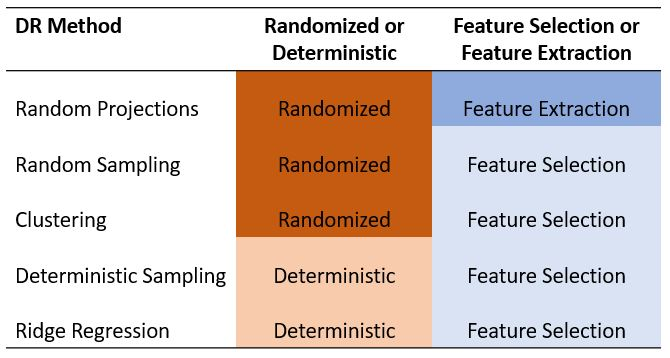
\includegraphics[scale=0.6]{figures/dim_red_methods_chart_2.JPG}
\caption{Summary of the five dimensionality reduction methods used in this paper. The methods are categorized as feature selection/feature extraction and as randomized/deterministic. }
\label{fig: dimRed_methods}
\end{figure}
\end{center}

\subsection{Background}
\label{sec:background}
Before we present the relevant literature for each of the DR methods, we review some key linear algebra definitions and notations. 

\begin{itemize}
\item We use $e_j$ to denote the $j$-th standard basis vector in  $\mathds{R}^n$, i.e., $e_j$ is a vector with its $j$-th entry equal to 1 and all other entries equal to 0.
\item Throughout this paper, $||\cdot||_2$ is  used to denote the spectral norm. We also use $||\cdot||_F$ to denote the Frobenius norm. The spectral and Frobenius norms of a matrix $\textbf{A} \in \mathds{R}^{m\times n}$ are defined as:

\begin{eqnarray*}
||\textbf{A}||_2 &=&  \sup_{x\in \mathds{R}^n, x\neq 0} \frac{|Ax|}{|x|},\ \text{and} \\
||\textbf{A}||_F &=& \sqrt{\sum_{i=1}^m \sum_{j=1}^n a_{ij}^2},
\end{eqnarray*}

where $a_{ij}$ are elements in matrix $\textbf{A}$ and $|\cdot|$ is the Euclidean vector norm defined as $|x| = \sqrt{\sum_{i=1}^n x_i^2}$. 

\end{itemize}

Statistical leverage scores have been an integral part of data analysis for many decades. They are a measure of how well the singular vectors of a matrix are correlated with the standard basis and thus have been used for outlier detection in regression analysis \cite{hoaglin_hat_1978, chatterjee1988}. Statistical leverages scores can also be interpreted as the amounted of leverage or influence a data point has \cite{velleman_efficient_1981}, and hence have found application in randomized matrix algorithms \cite{drineas_fast_2012, drineas_relative-error_2008, mahoney_cur_2009, drineas_faster_2011}. Leverage scores of the columns of a matrix are defined as the squared Euclidean norms of the columns of the matrix containing the top right singular vectors. More formally, \\

\textbf{Definition:} Given a matrix $\textbf{A} \in \mathds{R}^{n\times d}$, let $V'$ denote the matrix containing the top right singular vectors of $\textbf{A}$. Then, the statistical leverage score of the $i$-th column of $\textbf{A}$ is defined as,

\begin{equation}
l_i = \left\Vert V'_{(i)} \right\Vert_2^2 \ \ \forall\ i =1, 2,  \dots, d
\end{equation}

\noindent where $V'_{(i)}$ is the $i$-th column of the matrix $V'$. The computational bottleneck lies in the exact computation of $V'$, requiring $O(n^2d)$ time. This bottleneck can be avoided by calculating the relative-error approximations to the statistical leverage scores \cite{drineas_fast_2012}. \\


\subsection{Random Sketching}
\label{sec:random sketching}
In order to understand the need for a random sketching algorithm, let us consider the simple example of linear regression. Suppose we have a $ \textbf{X} \in \mathds{R}^{n \times d}$ full rank matrix of predictor variables and a response vector $\textbf{y}$ of length $n$. The least squares estimates can be computed as, 

\begin{equation*}
\hat{\beta} =  (\textbf{X}'\textbf{X})^{-1} \textbf{X}'\textbf{y}.
\end{equation*}

Thus, we need the Gram matrix $\textbf{X}'\textbf{X}$ and $\textbf{X}'\textbf{y}$ to compute the solution. The computation of $\textbf{X}'\textbf{X}$ requires $O(nd^2)$ time and $\textbf{X}'\textbf{y}$ requires $O(nd)$ time.  When $n > d$, this solution is easy to calculate and is very popular in practice. But, when $n, d$ or both are large --- as they tend to be in many modern data sets --- this computational time can be practically prohibitive. \\

Random sketching is a popular method to reduce the computational complexity of this problem.  Instead of using the full data set $(\textbf{X}, \textbf{y})$, we can employ a carefully constructed sketch $(\tilde{\textbf{X}},\tilde{\textbf{y}})$ to solve for the least squares coefficients. We define $\tilde{\textbf{X}} = \textbf{S}\textbf{X}$ and $\tilde{\textbf{y}}= \textbf{S}\textbf{y}$, where $\textbf{S}$ is a randomly generated ``sketching matrix" of size $r \times n$, $r << n$. The least squares solution will then be given by, 

\begin{equation*}
\hat{\beta_s} = (\tilde{\textbf{X}}'\tilde{\textbf{X}})^{-1} \tilde{\textbf{X}}'\tilde{\textbf{y}},
\end{equation*}

\noindent where $\hat{\beta_s}$ refers to the sketched solution. The cost of computing this solution reduces to $O(rd^2)$. For a sketched solution, our two primary goals are to ensure that the approximate solution is close to the original and to ensure that the computational time is significantly reduced. The careful construction of the sketching matrix $\textbf{S}$ helps us achieve both these goals. In the next section, we present the Johnson-Lindenstrauss Lemma and its role in random sketching algorithms. Following that, we explore literature to identify different choices for $\textbf{S}$ and their relative advantages and disadvantages.  \\

\subsubsection{Johnson-Lindenstrauss Lemma and its extensions}

Dimensionality reduction involves some form of mapping data from a high-dimensional space to a lower dimensional space in such a manner that the information from the original data is retained. The existence of a mapping that can approximately preserve pairwise distances while embedding data from a high-dimensional space into a lower-dimensional space was guaranteed by a lemma by \cite{JL1984} and is commonly known as the Johnson Lindenstrauss Lemma (JL Lemma). JL Lemma is a fundamental component of all random projection algorithms and hence we present a brief summary of the lemma and its extensions before discussing random projection. \\

\cite{JL1984} showed that $n$ points in an Euclidean space $\mathds{R}^d$ can be projected onto a $r= O(\log n /\epsilon^2)$ dimensional space without distorting any pairwise distances of the $n$ points by more than a factor of $(1\pm\epsilon)$ for any $\epsilon \in (0, 1/2]$. Johnson and Lindenstrauss provided this lemma as a tool to prove extensions of Lipschitz mapping into a Hilbert space. But due to its distance preserving nature, it has become a popular tool in dimensionality reduction. \\

\textbf{JL Lemma:} For any $\epsilon \in (0, 1/2]$ and any set of $n$ points $x_1, x_2, \dots, x_n$ in $\mathds{R}^d$, there exists a projection map $f: \mathds{R}^d \rightarrow \mathds{R}^r$, where $r= O(\log n /\epsilon^2)$. Then, for all $i,\  j \in \{1, 2, \dots, n\}$, 

\begin{equation}
(1-\epsilon)\Vert x_i-x_j \Vert_2^2 \leq \Vert f(x_i)-f(x_j)\Vert_2^2 \leq (1+\epsilon)\Vert x_i-x_j \Vert_2^2.
\end{equation}



Johnson and Lindenstrauss provided a lengthy technical proof using geometric approximation. Their main idea was summarized succinctly by  \cite{fedoruk_dimensionality_2018}:

\begin{itemize}
\item Project a set of points $x_1, x_2, \dots, x_n$ in  $\mathds{R}^d$ onto a random $r$- dimensional space. 
\item The expected length of each $r$-dimensional vector is $\sqrt{r/d}$ times the length of the original vectors. 
\item Multiplying each projection by  scaling factor of $\sqrt{d/r}$ yields $r$-dimensional vectors which are similar in length to the original $d$-dimensional vectors. 
\item If we choose a tolerance limit $\epsilon$, then with non-zero probability each length is preserved within the chosen tolerance limit. 
\end{itemize}

The JL Lemma has had numerous improvements and extensions over time. The improvements were two-pronged: improvements in the bounds for $r$ and improvements to the efficiency of $f(\cdot)$. The original proof by Johnson and Lindenstrauss suggested the lower bound for $r$ as $O(\log n /\epsilon^2)$. \cite{frankl1988} improved the lower bound to $r = O(9\log n /(\epsilon^2 - 2\epsilon^3/3))$. Further, they also provided a method to find a suitable mapping. JL Lemma only proves the existence of a mapping function $f(\cdot)$, but does not provide a way of finding one. \cite{dasgupta_elementary_2003} relied on probabilistic techniques to improve the lower bound results to $r= O(4\log n /(\epsilon^2/2 - 2\epsilon^3/3))$. Their proof is also considered significantly simpler than the original proof by \cite{JL1984}. Both these papers retained the definition of the random projection from the original paper, summarized below \cite{ailon_fast_2009} :

\begin{itemize}
\item Spherical symmetry: For any orthogonal matrix $A$, $A$ and $f(A)$ have the same distribution.
\item Orthogonality: The rows of $f(\cdot)$ are orthogonal to each other.
\item Normality: The rows of $f(\cdot)$ are unit-length vectors.
\end{itemize}

Improvements in the efficiency of $f(\cdot)$ were made through relaxing the assumptions listed above. \cite{har-peled_approximate_2012}  showed that the JL Lemma could be satisfied even without the  orthogonality and normality conditions being met. They proposed a projection matrix $R$ where each element of the matrix was sampled from the $N(0, 1/d)$ distribution. \\

\subsection{Random projection}

Random projection algorithms form one of the major class of random sketching algorithms. Random projection algorithms “uniformize” the non-uniformity structure present, by rotating the matrix to a basis where the uniform random sampling of features is nearly optimal. Random projection can be viewed as the process of dimensionality reduction with the objective of preserving the pairwise distances between observations. \\

Random projection produces matrices that are formed by a small number of linear combinations of all of the original features. The resulting compressed matrix can be used as a substitute in computations, thereby reducing the computational complexity of the problem at hand. The linear combinations are formed through pre-multiplying the features with a randomly generated coefficients matrix, and hence the name `random' projection. Given below is a simple random projection algorithm: 

\begin{itemize}
\item Consider an input matrix $\textbf{A} \in \mathds{R}^{n\times d}$ with $d >> n$ without loss of generality.
\item Construct a $d \times k$ random projection matrix $\textbf{S}$, where $k << n$.
\item Obtain the sketched matrix $\textbf{B}= \textbf{A}\textbf{S}$, where $\textbf{B}$ is a $n \times k$ matrix. 
\end{itemize}

\begin{center}
\begin{figure}[!t]
\centering
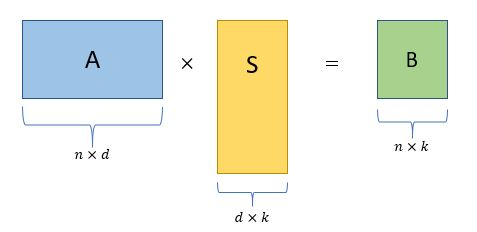
\includegraphics[scale=0.8]{figures/rp_1.JPG}
\caption{Schematic for a simple random projection.}
\label{fig:rp_scheme}
\end{figure}
\end{center}

Let us consider the example of performing the Singular Value Decomposition (SVD) of $\textbf{A}$. Using the original matrix $\textbf{A}$, the exact computation of SVD takes $O(nd^2)$ time. Instead, if we settle for an approximate SVD of $\textbf{A}$, we can compute the SVD of $\textbf{B}$ in place of $\textbf{A}$. The SVD computation on the smaller matrix $\textbf{B}$ takes only $O(nk^2)$ time even with the simple algorithm presented above. This example illustrates the motivation for using random projection as a tool for dimensionality reduction of large matrices. \\

There are two questions that come to mind quite naturally when looking at the algorithm presented above. How do we choose a suitable $\textbf{S}$ to obtain good approximations? For what values of $r$ will this algorithm produce good results? These two questions have been extensively studied over the last couple of decades and have lead to several candidates for the projection matrix $\textbf{S}$ and corresponding $r$ values. The JL Lemma (discussed in previous section) is fundamental in the construction of these projection matrices by providing the theoretical justification for the existence of a lower-dimensional subspace where the pair-wise distances between data points are preserved. We summarize some of the sketching matrices proposed in previous works:

\begin{itemize}


\item \textbf{Gaussian Sketch:} One of the first sketches proposed for random projection \cite{sarlos_improved_2006}. The sketch $\textbf{S}$ was formed by sampling each element from a Gaussian distribution $\textbf{S}_{ij} \sim N(0, 1/r)$, where $\textbf{S}_{ij}$ refers to the element in the $i$-th row and $j$-th column of matrix $\textbf{S}$.\\

\item \textbf{Rademacher Matrix:} \cite{achlioptas_fast_2007} proposed a simpler sketching matrix where each element of the matrix $\textbf{S}$ is a random variable taking $\{+1, -1\}$ with equal probability. Further, they also proved that a sparse matrix with $2/3$ of the entries replaced with 0 satisfies the Johnson-Lindenstrauss property.  This modification was an  important development, as the random matrix $\textbf{S}$ becomes a sparse matrix and leads to faster computations. \\

\item \textbf{FJLT:}  \cite{ailon_fast_2009} came up with the concept of fast Johnson-Lindenstrauss transforms (FJLT). The sketching matrix was generated as a product of three matrices $\textbf{S} = PHD$, where $P$ is a $r \times n$ sub-sampling matrix, $H$ is  a $n \times n$ dimension Hadamard matrix, and $D$ is a $n \times n$  random  diagonal matrix with entries taking values $\{+1, -1\}$ with equal probability. A Hadamard matrix is a square matrix with elements either $\{+1, -1\}$ and all the rows are orthogonal. \\

\item \textbf{CW Sketch:} The Clarkson and Woodruff sketch \cite{clarkson_low-rank_2017} is also a sparse matrix formed as a product of two independent random matrices $\textbf{S} = \Gamma D$, where $\Gamma$ is a $r \times n$ random matrix with only one element of each column set to $+1$ and $D$ is a $n \times n$ random diagonal matrix with entries taking values $\{+1, -1\}$ with equal probability. Thus,  $\textbf{S}$ will be a sparse random matrix with one non-zero entry in each of its columns. 
\end{itemize}

If the process of computing the lower-dimension projection was so computationally expensive that not much was gained on the whole, the whole exercise becomes futile. Thus, there has been significant research into building projection mappings that will enable efficient implementation of the random projection. Sparsification was a popular tool to reduce the number of computations performed during projection. \cite{achlioptas_fast_2007} were the first to propose a sparsified mapping to improve the speed of computation. They relaxed the spherical symmetry condition and proposed a projection matrix $R$ with each element independently taking values $\{+1,  -1\}$ with equal probability. The resulting projection satisfied the JL Lemma with lower bounds guarantees the same as the one proposed by \cite{dasgupta_elementary_2003}. Further, they showed that the JL Lemma and the lower bound guarantees hold even if the elements of $R$ are independently sampled from the distribution:

\begin{align*}
R_{ij}=
\begin{cases}
+\sqrt{3}, \ \ \ &\mbox{ with probability } 1/6 \\
0, \ \ \ &\mbox{ with probability } 2/3 \\
-\sqrt{3}, \ \ \ &\mbox{ with probability } 1/6 \\
\end{cases}
.
\end{align*} 

This result was especially important as $2/3$-rd of the elements of the projection matrix are 0 on average, which leads to faster computation. Achlioptas and Mcsherry (2007) noted that the $2/3$ proportion of 0s cannot be significantly improved without compromising the lower bound approximation guarantees. \cite{ailon_fast_2009} improved upon this aspect by proving that the sparsity of the projection matrix can be higher than $2/3$ if data points are well spread across the dimensions. They provided a method to construct sparse projection matrices for any data by using Fourier transforms. Their construction allowed for faster computation and they referred to the method as the Fast Johnson-Lindenstrauss Transform (FJLT). In this paper, we used the FJLT method for implementing the random projection method as it supports fast computation as well as requires modest amount of storage compared to other methods. \\

We now summarize the thought process followed in \cite{ailon_fast_2009}. Suppose we have an arbitrary vector $\textbf{x}$.  If $\textbf{x}$ was uniformly distributed, uniform random sampling and re-scaling can lead to a good estimate of the $l_2$-norm of $\textbf{x}$. But, often $\textbf{x}$ may not be uniformly distributed and thus uniform random sampling will lead to poor estimates of the $l_2$-norm. Uncertainty principle states that the more dense a function $f(\cdot)$, the more spread out its Fourier transformation and vice-versa. As a consequence of this, if $\textbf{x}$ is sparse then its Fourier transform $F\textbf{x}$ cannot be too sparse where $F$ is a Fourier transformation. By definition, a Hadamard transform is a multi-dimensional Fourier Transform. Hence, $H\textbf{x}$ also cannot be too sparse, where $H$ is a Hadamard transform. Despite this, $H\textbf{x}$ could still be sparse and so we re-randomize $H\textbf{x}$ with a cost-efficient rotation such as a diagonal matrix $D$ with its elements taking the values $\{+1, -1\}$ with equal probability. Finally, we use a sub-sampling matrix $P$ of size $r \times n$ which helps us sample from $HD\textbf{x}$. Thus, we have the final form of the FJLT given by $PHD\textbf{x}$. Due to the presence of the Hadamard matrix, this projection is also known as the Subsampled Randomized Hadamard Transform (SRHT). \\

Some of the key points to note from SRHT are:
\begin{itemize}
\item Since $D$ is diagonal, $D\textbf{x}$ can be computed in $O(n)$ time.
\item $H$ is applied to the n-dimensional vector $D\textbf{x}$ in $O(n\log n)$ time. 
\item $P$ is applied to an n-dimensional vector in $O(r)$ time.
\item Finally, the SRHT of a $n\times d$ matrix can be computed in $O(nd\log r)$ time. 
\end{itemize}

The Hadamard-based sketching scheme was particularly important for fast implementations of the random projection algorithms. FJLT was first proposed \cite{ailon_fast_2009} and was later applied to randomized algorithms in the form of SRHT \cite{sarlos_improved_2006, drineas_faster_2011}. The SRHT sketch was analyzed in detail by \cite{tropp_improved_2011}. Tropp also presented a simpler proof that the SRHT satisfies the JL property. \cite{boutsidis_improved_2013} improved upon this work and provided bounds for $r$ which have low dependence on  $n$. They also extended the results by applying SRHT for the approximation of matrix multiplication. \\

\subsubsection{Implementation of the random projection algorithm}

In this paper, we used the $RaProR$ package \cite{RaProR} in $\textbf{R}$ \cite{Rcite} to compute the random projection. The package was built based on theorems and results in \cite{geppert_random_2017}, which provides details about the algorithms implemented to compute the projection. In particular, the package allows for calculation of three kinds of sketching matrices: Rademacher matrix (RAD), Subsampled Randomized Hadamard Transform (SRHT), and Clarkson-Woodruff sketch (CW). From \cite{woodruff_sketching_2014, geppert_random_2017, ahfock_statistical_2019}, we can summarize a comparison of the sketches in terms of the sketching time and the corresponding value for $r$. The results are summarized in Table \ref{tab:sketch}. \\

\begin{table}[h]
\centering
\begin{tabular}{lll}
\hline
\textbf{Sketch}     & \textbf{Running Time}   & \textbf{Sketch size $(r)$}           \\
\hline
Gaussian   & $O(ndr)$       & $O(\{d+\log(1/\delta) \} \epsilon^{-2})$ \\
Rademacher & $O(ndr)$       & $O(\{d+\log(1/\delta) \} \epsilon^{-2})$ \\
SRHT       & $O(nd \log r)$ & $O(\{d \log (d/\delta)\}\epsilon^{-2})$  \\
CW         & $O(nd)$        & $O(d^2/\epsilon^2\delta )$              \\
\hline
\end{tabular}
\caption{Sketching time and necessary sketching size $r$ for different sketching schemes. The necessary sketch size $r$ refers to the minimum size such that the resulting random projection matrix satisfies the JL property with a probability of at least $(1-\delta)$.}
\label{tab:sketch}
\end{table}

As discussed earlier, we used the SRHT projection for our random projection implementation. The implementation of the random projection algorithm for dimensionality reduction of the genomic marker data set can be summarized as follows:

\begin{enumerate}
    \item Compute projection matrices with predefined  number of column $k$.
    \item Multiply the projection matrix with original marker data to obtain the reduced matrix $X$ of size $n \times k$.
    \item Use the reduced matrix to compute the genomic effect $G = XX'$ as input for the three genomic prediction models and obtain predictions in all three cross-validation schemes.
    \item Repeat steps 2-4 100 times to remove bias in the prediction results.
\end{enumerate}

The details about the prediction models and cross-validation schemes are given in section \ref{sec:gp and data}. The random projection implementation is visualized in Figure \ref{fig:rp_implement}. Like any feature extraction based DR method, the random projection method is based on the linear combinations of all of the original features. The newly created features may not be interpretable in the data scale. Even worse, they may have no practical meaning at all. For this reason, feature selection is an attractive alternative approach to dimensionality reduction. In feature selection, a subset of the original features are picked using various strategies. This allows for straightforward interpretation of results. In the next sections, we explore four different feature selection algorithms, starting with the random sampling algorithm which is the second approach to randomized sketching algorithms. \\

\begin{center}
\begin{figure}[!h]
\centering
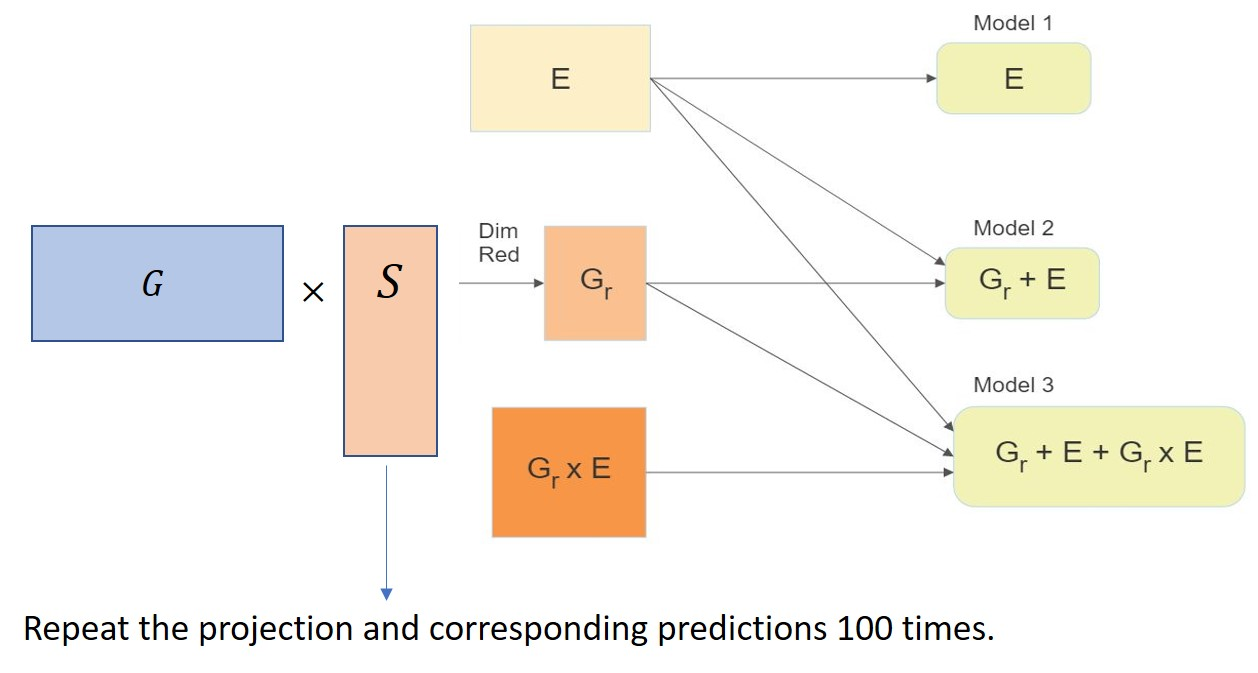
\includegraphics[scale=0.4]{figures/rp_2_1.jpg}
\caption{Implementation of the random projection algorithm for dimensionality reduction of the genomic data set in the genomic prediction problem.}
\label{fig:rp_implement}
\end{figure}
\end{center}

\subsection{Random Sampling}

Random sampling is another randomized approach to address the non-uniformity structure of data and form lower-dimension approximation matrices. While random projection addresses the non-uniformity by "uniformizing" the structure through rotations, random sampling algorithms build an importance probability to address the non-uniformity. We will describe the naive approach to random sampling followed by a simple random sampling algorithm. The naive random sampling algorithm does not apply any methods to bound the approximation error, but acts as an ideal introduction to these sampling algorithms. \\

The random sampling approach involves sampling a small number of features that represent the whole set of features. The naive approach randomly selects the features with uniform probability in independently and identically distributed (IID) trials. This approach ignores the non-uniformity structure presented in the data by giving an equal probability to each feature of the original predictor data. The reduced feature set could lose crucial information and structure from the original data. Hence, the naive uniform  sampling is not a popular choice of method for dimensionality reduction.\\

A more reasonable approach is to quantify the non-uniformity structure using some measure. Earlier, we had introduced statistical leverage scores. These leverage scores can be interpreted as a measure of influence the data points have on related computations and hence can be viewed as a metric to define the non-uniformity in the original matrix. Recall that the leverage score of the i-$th$ column of a matrix is given by $l_i = ||V'_(i)||_2^2$.
Since, $\sum_{i=1}^n l_i = ||V'||^2 = d$, we can define a probability distribution over the columns of $\textbf{A}$ given by $p_i = l_i/d$. We will refer to this probability distribution as the importance probability distribution which is a measure of the relative importance of columns in the matrix. It provides a probability distribution based on which the random sampling can be carried out while accounting for the non-uniformity structure of the original matrix. \\

As discussed earlier, the computational bottleneck for using importance probability distribution lies in its dependence on computation of the orthogonal basis for the input matrix. \cite{drineas_fast_2012} provided an algorithm to compute the relative-error approximate leverage scores $l_i$ instead of the computing the exact statistical leverage scores. Their contribution was a key development in the area of random sampling algorithms. We used their algorithm as the basis for implementing the random sampling algorithm in the genomic prediction problem. \\

We now describe the random sampling algorithm presented in \cite{drineas_fast_2012} along with drawing the attention of the reader to the salient properties and contributions. Consider a matrix $\textbf{A} \in \mathds{R}^{n \times d}$ with $d >> n$ and let $V'$ be the corresponding right singular matrix of $\textbf{A}$. Principally, we are interested in approximating the statistical leverage scores $l_i$ of the columns of $\textbf{A}$, which are then used to construct the importance probability distribution.

\begin{equation} \label{eq:2}
l_i = \left\Vert V'_{(i)}\right\Vert_2^2 = \left\Vert e'_i\ V' \right\Vert_2^2
\end{equation}

\noindent where $e_i$ is the $i$-th standard basis vector. The computation of the orthogonal matrix $V'$ takes $O(n^2d)$ time, which is the bottleneck. Since $V'$ can also be seen as any orthogonal basis for the column space of $\textbf{A}$, it follows that $V'V = AA^+$ where $^+$ is the Moore-Penrose inverse. From this, we can redefine the statistical leverage scores as,

\begin{equation} \label{eq:3}
l_i = \left\Vert e'_i\ V' \right\Vert_2^2 = \left\Vert e'_i\ V'V \right\Vert_2^2 = \left\Vert e'_i\ AA^+ \right\Vert_2^2.
\end{equation}

The computational complexity of calculating the leverage scores according to Eqn. \ref{eq:3} involves computing the pseudo-inverse $\textbf{A}^+$ and performing the matrix multiplication of $\textbf{A}$ and $\textbf{A}^+$. We apply random projection to overcome both these complexities by performing the computations and finally obtaining the approximate leverage scores $\tilde{l}_i$. \\ 

Instead of computing $\textbf{A}^+$, we find a smaller matrix that approximates $\textbf{A}$ and find the corresponding Moore-Pensore inverse of the smaller matrix. Subsampled Randomized Hadamard Transform (SRHT) is used to derive the smaller matrix as it preserves the structure $\textbf{A}$. SRHT rotates $\textbf{A}$ to a random basis where all the rows have an equal influence and uniformly samples rows from that basis. If $\Pi_1 \in \mathds{R}^{r_1 \times n}$ is a $\epsilon$-FJLT matrix for $V'$, then $\Pi_1 \textbf{A}$ is the approximation of $\textbf{A}$. Then Eqn. \ref{eq:3} becomes,

\begin{equation} \label{eq:4}
\hat{l}_i = \left\Vert e'_i\ A(\Pi_1 A)^+ \right\Vert_2^2.
\end{equation}

While computing the product $\textbf{A}\textbf{A}^+$ takes $O(nd^2)$, the computation of $\textbf{A}(\Pi_1 \textbf{A})^+$ takes $O(ndr_1)$ time. This is not efficient since $r_1 > d$. Since only the Euclidean norms of the rows of $\textbf{A}(\Pi_1 \textbf{A})^+$ are required, the dimensionality of this matrix can be reduced by using a $\epsilon$-JLT for the rows of $\textbf{A}(\Pi_1 \textbf{A})^+$. Suppose $\Pi_2 \in \mathds{R}^{r_1 \times r_2}$ is an $\epsilon$-JLT, then $\textbf{A}(\Pi_1 \textbf{A})^+ \Pi_2$ is a randomized sketching of $\textbf{A}\textbf{A}^+$. Then we can compute the approximate statistical leverage scores as

\begin{equation} \label{eq:5}
\tilde{l}_i = \left\Vert e'_i\ A(\Pi_1 A)^+\Pi_2 \right\Vert_2^2.
\end{equation}

 \cite{drineas_fast_2012} showed that for any error parameter $\epsilon \in (0, 0.5]$ and any arbitrary matrix $\textbf{A}$ of size $n \times d$ with $n >> d$, the expression 

\begin{equation}
|l_i - \tilde{l}_i| \leq \epsilon l_i 
\end{equation}
 holds for all $i = 1, 2, \dots, n$. \\

This result can be  extended without loss of generality for $d >> n$ case as well. \cite{ma_statistical_2015} investigated the approximation quality for several combinations of $r_1$ and $r_2$ through simulation studies. They found that $r_1$ does not have a significant impact on the correlation between approximate and exact leverage scores but running time increases linearly with $r_1$. On the other hand, the correlations between approximate and exact leverage scores increase rapidly with increasing $r_2$, but $r_2$ does not impact running time. Thus, they concluded that a combination of small $r_1$ and large $r_2$ would result in high-quality approximations with short run time. \\

\subsubsection{Implementation of the random sampling algorithm}

We used the statistical leverage scores to calculate the importance probability distribution required for the random sampling algorithm. We followed the two stage algorithm presented by \cite{boutsidis_improved_2009} to implement the random sampling algorithm. The implementation of the random sampling algorithm for dimensionality reduction of the marker data set for genomic prediction is as follows:


\begin{enumerate}
    \item Compute the approximate leverage scores as defined in \cite{drineas_fast_2012}.
    \item Use the approximate leverage scores to define the importance sampling distribution for the columns of the input marker matrix $X$.
    \item Randomly sample predefined number of columns $k$ according to the importance sampling distribution to form reduced matrices of different sizes.
    \item Use the reduced matrix $X$ to compute the genomic effect $G = XX'$ as the input for the prediction models and obtain predictions in all cross-validation schemes. 
    \item Repeat steps 3-4 100 times to remove sampling bias from the prediction accuracy results.  
\end{enumerate}

The advantage of this random sampling algorithm is the computation of the approximate leverage scores instead of the exact scores, effectively reducing computation time. In the next section, we describe another randomized algorithm for dimensionality reduction based on clustering. \\


\subsection{Clustering}
\label{sec:clustering}

Clustering is the process of grouping a set of objects in such a way that objects in the same group are more similar to each other than to objects in different groups, called clusters. Grouping objects when the data are labeled is a trivial task and is often referred to as supervised classification \cite{jain_data_1999}. But, often we are presented with data with no labeling available. Clustering was developed as a tool to deal with problems where the objective was to group unlabeled objects into meaningful collections. Because of the absence of labels, clustering is also called as unsupervised classification. \\

Clustering has seen immense interest in recent decades through its various applications in pattern and object recognition, recommender systems, and machine learning. It was first introduced in anthropology by Driver and Kroeber (1932) where they grouped cultures from different tribes of Polynesia and the Americas based on the presence or absence of traits such as matrilineage, sinew-backed bow, twined weaving, ridged houses, etc. Over the years clustering has been applied as a classification tool in many fields such as social science, psychology, biology, marketing, medicine, etc \cite{Hartigan1975, Punj1983, Jiang2004, Clatworthy2005, Sutherland2012}. Clustering is also used for detecting anomalies in the data, for identifying degree of similarity of objects, and for organizing and summarizing data. \\

The general scheme of clustering is to start with $n$ objects and sort them into $K$ groups based on some similarity measure such that the intra-group similarity is high and the inter-group similarity is low. Several categorizations of the clustering algorithms are available. Clustering algorithms can be broadly divided into partitional and hierarchical algorithms \cite{fraley_model-based_2002}. \cite{xu_comprehensive_2015} classified the clustering algorithms into traditional and modern each with 9 categories and 10 categories, respectively. Developing clustering algorithms is not the focus of this paper, so we will discuss only partitional and hierarchical clustering algorithms and use them as a means to compare clustering to the other dimensionality reduction algorithms. \\

\subsubsection{Partitional Clustering Algorithm}

Partitional clustering divides the set into non-overlapping subsets (clusters) such that each object is present only in one cluster. Typically, partitioning clusters produce clusters by optimizing some criterion function to produce optimal solutions \cite{Hartigan1975}. K-means, the most popular partitional algorithm, is an algorithm  where the objective is to minimize the sum of the squares of the distances from the objects to the centroid of the cluster. K-means algorithm ensures that there are always exactly $k$ clusters at the end of the process, with each cluster containing at least one item. \\

The general form of the k-means algorithm is as follows:

\begin{enumerate}
\item Choose the number of cluster, $k$.
\item Randomly assign $k$ out of $n$ items as cluster centroids.
\item Assign all the remaining $(n-k)$ items in the collection to their nearest cluster based on distance to the centroid.
\item Recompute the cluster centroids based on the current cluster assignment. 
\item Reassign items to their nearest cluster based on distance to centroids.  
\item Repeat steps 4-5 until no items change cluster assignments, or an iteration threshold is met. 
 \end{enumerate}

K-means clustering is a very efficient and easy algorithm to apply. However, it may not be a suitable algorithm in certain cases:

\begin{itemize}
\item \textbf{Non-globular cluster:} The solution to the k-means clustering is obtained by minimizing the within-cluster sum of squares. This is minimized when the clusters are globular and when the clusters are well separated from each other. Thus, applying k-means to non-globular shapes leads to results that are not optimal. Non-globular clusters can be visualized as in Figure \ref{fig:nonglob}.

\item \textbf{Non-uniform cluster sizes:} The cluster sizes are expected to be more or less similar to each other. K-means algorithm is not suitable when there is large variation in the cluster sizes from one cluster to the next. This issue is depicted in Figure \ref{fig:diffsizes}.

\item \textbf{Presence of outliers:} K-means algorithm is sensitive to outliers. The algorithm updates the centroids of the clusters by taking the average of all the points in the cluster. The presence of outliers will pull the centroid towards the outliers and lead to mis-classification of data points into the wrong clusters. There are several solutions in the literature to perform k-means in the presence of outliers \cite{dave_robust_1997, gan_k_2017, jiang_giniclust_2016, hautamaki_improving_2005}.

\begin{figure}[!htp]
  \centering
  \subfloat[Non-globular clusters]{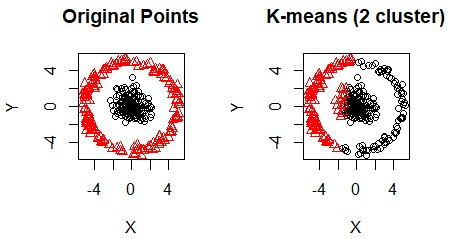
\includegraphics[width=0.5\textwidth]{figures/kmeans2_compiled.jpg}\label{fig:nonglob}}
  \hfill
  \subfloat[Non-uniform cluster sizes]{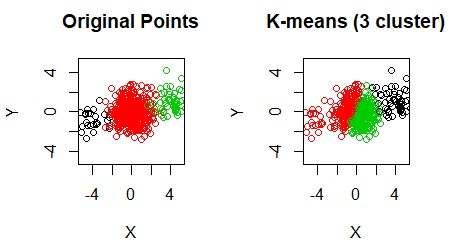
\includegraphics[width=0.5\textwidth]{figures/kmeans1_complied.jpg}\label{fig:diffsizes}}
  \caption{Limitations of K-means algorithm\\}
\end{figure}

\end{itemize}

Some of the drawbacks such as the need for globular clusters and the need for cluster sizes to be similar can be overcome by using a hierarchical clustering approach rather than a partitional clustering algorithm. We expand on the hierarchical clustering method in the next section. 

\subsubsection{Hierarchical Clustering Algorithm}

Hierarchical clustering is the process of creating a set of nested clusters arranged into a tree or dendrogram structure. Hierarchical clustering does not require a determination of the number of clusters $k$ prior to the clustering process, as opposed to the k-means clustering. The nested structure provides flexibility of choosing the number of clusters based on the dendrogram as well as domain expertise \cite{jain_data_1999}. There are two possible directions of clustering under hierarchical clustering: agglomerative (bottom-up) and divisive (top-down). In agglomerative clustering, each object is a cluster by itself initially and the most similar clusters are paired together successively to form a hierarchy. In divisive clustering, we start with the entire set of objects as one cluster and recursively divide each cluster into sub-clusters based on dissimilarity. Both these approaches lead to a hierarchy among objects which can be represented by a dendrogram. In this paper, we focus only on the agglomerative hierarchical clustering approach. A typical agglomerative hierarchical clustering scheme is given below:

\begin{enumerate}
\item Start with each item in its own cluster. 
\item Compute all similarity between all pairs of clusters. 
\item Merge the two clusters that are most similar to each other based on the clustering metric.
\item Repeat the process until only one cluster is remaining.
\end{enumerate}

The process of merging clusters at each iteration leads to a dendrogram depicting the hierarchy structure present. The merging of clusters is determined by clustering metrics which define the similarity among the clusters. There are several clustering metrics available in literature, some of which are presented in the next section. 

\subsubsection{Clustering Metrics}

There are several metrics that can be used to compute the similarity or dissimilarity between clusters. In this paper, we describe four of the most popular metrics: single-linkage \cite{sneath_numerical_1973}, complete-linkage \cite{king_step-wise_1967}, average-linkage \cite{eslr} and Ward's method \cite{murtagh_survey_1983, ward_hierarchical_1963}. \\

\textbf{Single-linkage}, also known as minimum linkage, method computes all pairwise distance between the elements within two clusters, and considers the smallest of these distances as a linkage criterion. The single-linkage algorithm is versatile in applications, but often tends to produce elongated clusters. To merge two clusters using single-linkage, only one object of the cluster needs to be close to the other cluster. Thus, this could lead to chaining and elongated clusters. Single-linkage also does not perform well if there is noise between clusters. In other words, single-linkage is not suitable if the clusters are not well separated. \\

\textbf{Complete-linkage} method considers the largest value (i.e., maximum value) of these distances as the distance between the two clusters. Complete-linkage method tends to produce more compact clusters and is also less susceptible to outliers and noise. It produces well-bounded compact clusters compared to single-linkage method, but tends to break large clusters into smaller ones. \cite{Jain1988} observed that complete-link is often the sensible option in most applications. \\

\textbf{Average-linkage} method computes all pairwise distances between elements in two clusters and takes the average of all distances as the distance between the two clusters. Average-linkage algorithm also performs well in the presence of noise between clusters. But like the complete-linkage algorithm, it tends to produce globular clusters. \\

\textbf{Ward's method}, or Ward's minimum variance method, computes the distance between two clusters as the increase in the total within-clusters sums of squares when two clusters are merged. The two clusters whose union leads to the smallest increase in the sum of the squares are merged together. Ward's method has the same disadvantages as complete-linkage, whereby it favors globular clusters. \\

Single-linkage is not the preferred metric due to its susceptibility to produce elongated clusters. Complete-linkage is avoided because of its inability to retain large clusters. Between average-linkage and Ward's minimum variance method, there is no real distinguishing factor. Since Ward's method can be compared easily to the objective function in k-means, we picked the Ward's method as our metric of choice for the hierarchical clustering approach.

\subsubsection{Implementation of clustering for dimensionality reduction}

In this section, we describe our approach to applying dimensionality reduction to genomic data sets with clustering acting as the reduction technique. Hierarchical clustering creates a nested clustering structure, often represented by a dendrogram. This allows the user to create any number of clusters by choosing the appropriate height to cut the dendrogram. One of our objectives was to study the trend in prediction accuracy as a function of the input data sizes. Thus, we are interested in creating reduced data sets of 26 different sizes. The K-means algorithm needs to be run 26 times to obtain the 26 different reduced marker data sets. On the other hand, hierarchical clustering needs to be performed only once to determine the hierarchy. The 26 different marker data sets can be created by cutting the dendrogram 26 times at appropriate heights. Thus, hierarchical clustering is computationally more efficient for our application and hence is the clustering algorithm of choice for this paper. \\

The R package $`fastcluster'$ \cite{mullner_fastcluster_2013} was used for fast implementation of the hierarchical clustering algorithm. The implmentation of the clustering algorithm for dimensionality reduction of the genomic data set can be summarized as follows:

\begin{enumerate}
    \item Perform agglomerative hierarchical clustering using $`fastcluster'$ to determine the hierarchy.
    \item Form $k$ clusters from the hierarchy by cutting appropriately.
    \item Sample one feature randomly from each of the $k$ clusters as the representative of that cluster.
    \item The sampled features form the reduced data set of size $k$ and will be used for the genomic prediction models.
    \item Repeat the sampling from the clusters and the following model implementation 100 times to remove sampling bias in the prediction accuracy results. 
\end{enumerate}

In the next sections, we describe two deterministic feature selection algorithms. First, we look at the deterministic sampling algorithm which is a deterministic analogue of the random sampling algorithm. 

\subsection{Deterministic Sampling}
\label{sec:det_sampling}

The feature selection method involves selecting a small subset of the original features to create the compressed feature matrix and hence avoids the issues with inference and  interpretability. Feature selection is also known as the column subset selection problem (CSSP) in matrix theory and linear algebra. Before we discuss the feature selection based dimensionality reduction approach in greater detail, we define CSSP formally.\\

\textbf{Column Subset Selection Problem: } Let $\boldsymbol{A} \in \boldsymbol{\mathds{R}}^{n \times d}$ and let $c < d$ be a positive integer. Select $c$ columns of A to form a matrix $\boldsymbol{C} \in \mathds{R}^{n \times c}$ that minimizes 

\begin{equation}
\left\Vert A - CC^+A \right\Vert_\xi 
\end{equation}

\noindent where $\textbf{C}^+$ denotes the Moore-Penrose inverse \cite{penrose_generalized_1955} of matrix $\textbf{C}$ and $\xi = \{2, F\}$, denotes the spectral or Frobenius norm \cite{meyer2000}, respectively. \\

Jolieffe \cite{jolliffe_discarding_1972} proposed one of the first column subset selection algorithms. The algorithm involved deterministic sampling of the columns of the matrix based on ordered leverage scores. While the algorithm led to favorable dimensionality reduction in many practical applications, they did not provide theoretical guarantees on the quality of the approximation and hence, it was not widely used. \cite{drineas_relative-error_2008} developed the randomized counterpart to the deterministic sampling algorithm that employs a sampling probability distribution based on the leverage scores. They proved that their algorithm produces a matrix $C$ that satisfies $\left\Vert A - CC^+A \right\Vert \leq (1+\epsilon) \left\Vert A - A_k \right\Vert $ with constant probability and hence guaranteed the approximation quality of their algorithm. Here, $A_k$ is the best rank-k approximation obtained from SVD and $c = O(k \log k / \epsilon^2)$ is the number of columns in $C$. \\

The randomized algorithm gives a `near-optimal' approximation of the matrix, but may not be computationally as efficient as the deterministic algorithm.  \cite{papailiopoulos_provable_2014} developed theoretical derivations for the approximation errors of the deterministic sampling algorithm provided by \cite{jolliffe_discarding_1972}. They proved that if the ordered leverage scores $l_i$  follow a steep enough power-law decay, then the deterministic algorithm performs equally or better than the randomized algorithm. Further, if the leverage scores follow a steep power-law decay, then the number of columns chosen by the deterministic algorithm is similar or fewer than the randomized counterpart as proposed by \cite{drineas_relative-error_2008}. They showed the utility of the power-law decay assumption by providing several examples of real data sets where the leverage scores followed a power-law decay. \cite{papailiopoulos_provable_2014} also emphasized that while their theoretical analysis was performed for the power-law decay model, other models for the leverage scores could be developed. \\

We now summarize the deterministic algorithm presented in \cite{papailiopoulos_provable_2014} as well as briefly state the theorems that guarantee the quality of the approximations produced from this algorithm. The proofs for the theorems are beyond the scope of this paper and detailed presentation of the proofs can be found in \cite{papailiopoulos_provable_2014}. \\

\noindent The deterministic algorithm can be described in 3 steps:

\begin{enumerate}
    \item Compute the top-$k$ right singular vectors $\textbf{V}_k$ of $\textbf{A}$ using SVD of $\textbf{A}$.
    \item Calculate the leverage scores $l_i^{(k)}$,  where the superscript refers to the choice of $k$ in the SVD. Reorder the leverage scores in a decreasing order. 
    \item Select $c$ columns of $\textbf{A}$ that correspond to the top $c$ leverage scores such that their sum is greater than some stopping threshold $\theta$, $\sum_{i=1}^c l_i^{(k)}>\theta$. The choice of $\theta$ controls the quality of the approximation. 
\end{enumerate}


\begin{algorithm}[t]
\SetAlgoLined
\KwIn{$\textbf{A} \in \mathds{R}^{n\times d}$, $k$, $\theta$}

1: Compute $A = U\Sigma V^T$, the singular value decomposition of $\textbf{A}$. Extract the top-$k$ right singular vectors of $\textbf{A}$, $\textbf{V}_k \in \mathds{R}^{d \times k}$.\\
2: \For{$i \gets 1$ \textbf{to} $d$} {
	$l_i^{(k)} = \left\Vert [V_k]_i, \right\Vert_2^2$
}
3 : Without loss of generality, let the leverage scores be sorted in decreasing order:
\begin{equation}
l_1^{(k)} \geq l_2^{(k)} \geq \cdots \geq l_d^{(k)}. \notag
\end{equation}
Sort the columns of $\textbf{A}$ according the leverage scores. Let the sorted column indices be $\pi_i$.\\ 
4: Find $c \in {1, 2, \cdots, n}$ such that 
\begin{equation}
c  = arg\min_c \left(\sum_{i = 1}^c l_i^{(k)} >\theta \right). \notag
\end{equation} 

5.  If $c<k$ from step 4, we set $c = k$. \\
6. Construct a subsampling matrix $\textbf{S} \in \mathds{R}^{d \times c}$. If the column $\pi_i$ is selected, then $S_{i,  \pi_i} = 1$ and 0 otherwise. \\
\KwOut{$\textbf{S} \in \mathds{R}^{d \times c}$ such that $C = AS$ contains top $c$ columns of $\textbf{A}$.}
 \caption{Deterministic Sampling Algorithm}
\end{algorithm}

The deterministic sampling algorithm requires the implementation of SVD to compute the leverage scores. Hence, the time complexity of the algorithm is given by $O(nd \min({n,d}))$. The resulting matrix from the deterministic sampling algorithm guarantees a bound on the approximation error with regard to the CSSP. This result is summarized in the following theorem whose proof can be found in \cite{papailiopoulos_provable_2014}. \\

\begin{theorem}[Deterministic Sampling]
Let $\theta = k - \epsilon$ for some $\epsilon \in (0,1)$. For a matrix $\textbf{C}$ obtained from the deterministic sampling algorithm and for $\xi = \{2,F\}$, we have
\begin{equation}
\label{eqn:thm1}
\left\Vert A - CC^+A \right\Vert_\xi^2 < (1-\epsilon)^{-1}\cdot \left\Vert A-A_k  \right\Vert_\xi^2. 
\end{equation}
\end{theorem}

In other words, the deterministic sampling theorem (DS theorem) shows that when a compressed matrix is derived using the deterministic sampling algorithm, the approximation error is at most $(1-\epsilon)^{-1}$ times the best approximation error obtained by the SVD method. DS theorem proves the existence of a high quality approximation matrix using the deterministic sampling algorithm and provides bounds for the possible values of $c$. More specifically, it dictates that the number of columns sampled is at least $k$, i.e., $c \geq k$. In the worse case scenario where the leverage scores follow a uniform distribution, the number of columns required to be sampled approaches $d$, where d is the total number of columns in the original matrix. \cite{papailiopoulos_provable_2014} further state that when the leverage scores exhibit a power-law decay, the number of columns selected by the deterministic sampling algorithm can be determined exactly. This is stated formally in the following theorem. 


\begin{theorem}[Power Law]
Let the leverage scores follow a power-law decay of the form:
\begin{equation}
\label{eqn:powerlaw}
l_i^{(k)} = \frac{l_1^{(k)}}{i^{\alpha_k}}
\end{equation}
where, $\alpha_k = 1+\eta$ for $\eta >0$. If we set the stopping threshold $\theta = k-\epsilon$ where $0<\epsilon<1$,  then the number of columns sampled by Algorithm 1 is:
\begin{equation}
c = \max \left\{\left( \frac{2k}{\epsilon} \right)^{\frac{1}{1+\eta}}-1, \ \ \left( \frac{2k}{\eta \cdot \epsilon} \right)^{\frac{1}{\eta}}-1,\ \  k \right\}.
\end{equation}

\end{theorem}

The corresponding subsampled matrix $\textbf{C}$ achieves the approximation error given in Eq. \ref{eqn:thm1}. \\

The deterministic sampling algorithm depends on two input parameters, $k$ and $\epsilon$. The parameter $k$ determines the rank of the SVD approximation of A, and the parameter $\epsilon$ determines the error tolerance when comparing $\textbf{C}$ to $\textbf{A}_k$ from SVD. The implementation of the deterministic algorithm for the purpose of genomic prediction can be seen as a pre-processing step. Given a large genomic information matrix, we use the deterministic algorithm to create a compressed matrix that represents the whole matrix well. \\

\subsubsection{Implementation of the deterministic sampling algorithm}

The deterministic sampling algorithm implementation mimics the random sampling implementation without the randomized sampling based on the leverage scores. The deterministic sampling algorithm can be summarized as follows:

\begin{enumerate}
    \item Compute the approximate leverage scores as defined in \cite{drineas_fast_2012}.
    \item Arrange the leverage scores in decreasing order. 
    \item Pick the top $k$ leverage scored columns to form the reduced matrices.
    \item Use these reduced matrices as the input for the genomic prediction models. 
\end{enumerate}


\subsection{Shrinkage Methods}
\label{sec:shrinkage methods}
Variable selection is the process of choosing a subset of the explanatory variables to explain a response variable. Variable selection helps in making models easier to interpret, reducing noise introduced by redundant variables, and reducing the size of the data set for faster computations. For these reasons, variable selection proves to be an important step in the analysis of high-dimensional data where the implementation and interpretation of models are made difficult due to the large number of variables present. \\


When the number of variables is very large, traditional subset selection methods have significant drawbacks. The best subset selection method involves fitting separate models for each possible combination of the $p$ predictors. For a problem with $p$ predictors, there are $2^p$ possible subset selections. The task of finding the "best" subset is practically unfeasible as $p$ increases. Stepwise selection methods are an alternative to the best-subset-selection method. They fit only a restricted set of models as opposed to the best-subset-selection method. Forward and backward stepwise selection are the two popular stepwise  selection algorithms. Both evaluate only $1+p(p+1)/2$ models compared to the $2^p$ models that are evaluated by best-subset-selection. Even though both these algorithms do not guarantee finding the "best" model containing a subset of the $p$ predictors, they are known to perform well in practice \cite{james_introduction_2013}. In high dimensional problems where $p > n$, backward selected cannot be used because of the initialization of the algorithm by fitting the full model. Forward selection can be used even when $ p > n$ as its initialization depends on fitting the null model containing no predictors. \\

Another drawback of the  traditional subset selection methods is the discrete nature of the variable selection, i.e., the variables are either retained or discarded. This leads to unstable variable selection, where a small change in data can lead to large change in the subset selected \cite{breiman_heuristics_1996}. Shrinkage methods were developed to address the shortcomings of the subset selection methods. These methods are also known as regularization or penalized methods. They work on the principle of imposing a constraint term that penalizes for model complexity. Shrinkage methods help in variable selection as well as improving the model's prediction performance through the bias-variance trade-off. In other words, shrinkage methods may provide solutions that have lower variance and higher bias, but ultimately leading to better prediction accuracy according to the mean squared error (MSE). \\

In this paper, we investigate the shrinkage methods as a tool for variable selection. We use the coefficients of the predictors, obtained from the shrinkage methods, as a form of ranking for variable selection. Our objective is to study how well the predictors are able to explain the response, as the number of predictors selected increases. In the following section, we describe the three popular shrinkage methods - LASSO, ridge regression, and elastic net  - along with their respective advantages and drawbacks. \\

\subsubsection{Ridge Regression}

Consider a standard linear regression model, 

\begin{equation}
y_i = \beta_0 + \sum_{j = 1}^p \beta_j X_{ij} + \epsilon \notag
\end{equation}

\noindent where $y_i$ is the response value for the $i$-th observation, $X_{ij}$ represents the $j$-th predictor for the $i$-th observation, and $\beta_j$ is the coefficient of the $j$-th predictor. The coefficients $\beta_j$ can be estimated as the values that minimize the residual sum of squares (RSS) function, 

\begin{equation}
RSS = \sum_{i = 1}^n \left( y_i - \beta_0 - \sum_{j = 1}^p \beta_j x_{ij} \right)^2.
\end{equation}

The estimates obtained by minimizing the RSS are known as the ordinary least squares (OLS) estimates. The OLS estimates are reliable only if the predictors are orthogonal. Further, if we have a high-dimensional problem with $p > n$, then OLS does not have a solution. Ridge regression was proposed by Hoerl and Kennard in 1970 as a solution to problems where OLS estimates are unreliable \cite{hoerl_ridge_1970}. While OLS estimates are unbiased, ridge regression estimates are biased. But, the increase in bias is compensated by a decrease in variance and results in estimates with smaller MSE. \\

Ridge regression is similar to least squares regression, but the estimates are obtained by minimizing a different objective function. In OLS, the coefficients are estimated by minimizing the RSS function. In ridge regression, the coefficients $\beta_j$ are estimated by minimizing a penalized residual sum of squares, 

\begin{equation}
\sum_{i = 1}^n \left( y_i - \beta_0 - \sum_{j = 1}^p \beta_j x_{ij} \right)^2 + \lambda \sum_{j = 1}^p \beta_j^2 = RSS +  \lambda \sum_{j = 1}^p \beta_j^2,
\end{equation}

\noindent where $\lambda\geq 0$ is a penalty parameter. $\lambda\sum_{j =1}^p \beta_j^2$ is called the penalty term and we note that it takes an $L_2$ penalty form. $\lambda$ controls the amount of shrinkage of the parameters $\beta_j$. The larger the penalty parameter, the greater the amount of shrinkage and the greater the coefficients are shrunk towards 0. When $\lambda=0$, the ridge regression estimates are equal to the OLS estimates. At $\lambda = 0$, the variance is high and the bias is low. As $\lambda$ increases, the variance reduces substantially but the bias increases only marginally. Thus, ridge regression provides equally or more accurate predictions compared to OLS regression. Further, if $p>n$, OLS does not provide unique solution whereas ridge regression can perform well by exploiting the bias-variance trade-off. \\

In ridge regression, the penalty parameter has to be estimated separately. There are several methods for estimating the most appropriate penalty parameter $\lambda$. The most popular and reliable method is cross-validation. We can choose a range of $\lambda$ values, compute the cross-validated error for each value of $\lambda$ and pick the $\lambda$ corresponding to the smallest cross-validation error \cite{james_introduction_2013}. Another method is to pick $\lambda$ by an automated procedure as proposed by \cite{hoerl_ridge_1975}. They proposed selecting the value of the penalty parameter as $\lambda = \frac{rs^2}{\sum_{j = 1}^p \hat{\beta}_j^2}$, where $r$ is the number of parameters in the model, $s^2$ is the RSS from the least squares estimation, and $\hat{\beta}_j$ are the least square estimates of the regression coefficients. \\
 
Ridge regression uses all the $p$ predictors in the final model. The term $\lambda\sum_{j = 1}^p \beta_j^2$ shrinks all coefficients towards 0, but does not set any of them exactly equal to zero. Hence, none of the predictors are removed from the final model. This can be perceived as a disadvantage in the context of the variable selection problem. In this paper, our focus is on reducing the dimensionality of the data using variable selection. Both subset-selection and dimension reduction methods lead to reducing the number of predictor variables used in the final model. Thus, another shrinkage method called Least Absolute Shrinkage and Selection Operator (LASSO) was proposed by  Tibshirani in 1996 \cite{tibshirani1996} that overcomes this disadvantage and allows the shrinkage to be 0. \\ 

\subsubsection{LASSO}

LASSO is a shrinkage method that applies an $L_1$ penalty on the regression coefficients. In ridge regression, an $L_2$ penalty was applied. Due to the nature of the $L_1$ penalty, LASSO performs both shrinkage and automatic variable selection \cite{tibshirani1996}. In other words, the penalty term not only shrinks the coefficients towards 0, it sets some of the coefficients to 0. Thus, LASSO inherently `eliminates' the predictors from the final model that have coefficients 0, . \\

In ridge regression, the coefficients are estimated by minimizing a penalized residual sum of squares with a $L_2$ penalty. With LASSO, the coefficients $\beta_j$ are estimated by minimizing a penalized residual sum of squares with an $L_1$ penalty:

\begin{equation}
\sum_{i = 1}^n \left( y_i - \beta_0 - \sum_{j = 1}^p \beta_j x_{ij} \right)^2 + \lambda \sum_{j = 1}^p | \beta_j | = RSS +  \lambda \sum_{j = 1}^p | \beta_j | ,
\end{equation}

\noindent where $\lambda \geq 0$. When the penalty parameter $\lambda$ is sufficiently large, some of the coefficient estimates are set to be exactly equal to 0. A detailed explanation of why LASSO sets some coefficients to 0 while ridge regression does not, can be found in \cite{tibshirani1996} and \cite{james_introduction_2013}. Thus, LASSO performs variable selection. As with the ridge regression, when $\lambda  = 0 $ the LASSO estimates are equivalent to the OLS estimates. The penalty parameter $\lambda$ has to be estimated separately, similar to ridge regression. The cross-validation method of searching for optimal value of $\lambda$ works with LASSO as well and is the most popular one. \\

LASSO has its own set of disadvantages. When $p>n$, LASSO selects at most $n$ variables \cite{zou_regularization_2005}. Further, LASSO selects only one variable at random from a group of high correlated variables. This can be a significant drawback in situations where selecting one of the variables from the group implies that all other variables are important as well because LASSO selects only one and discards the rest of the variables in the group. \cite{zou_regularization_2005} proposed a new shrinkage method called the elastic net to overcome the problems presented by LASSO while retaining the advantages of LASSO. \\


\subsubsection{Elastic Net}

Elastic net can be viewed as a combination method involving both ridge regression and LASSO \cite{zou_regularization_2005}. In elastic net, the coefficients $\beta_j$ are estimated by minimizing a penalized residual sum of squares with an elastic net penalty term:

\begin{eqnarray}
\sum_{i = 1}^n \left( y_i - \beta_0 - \sum_{j = 1}^p \beta_j x_{ij} \right)^2 &+& \lambda \sum_{j = 1}^p \left( (1-\alpha) |\beta_j| + \alpha \beta_j^2 \right) \notag \\
= RSS &+&  \lambda \sum_{j = 1}^p \left( (1-\alpha) |\beta_j| + \alpha \beta_j^2 \right) ,
\end{eqnarray}

\noindent where $\alpha = \frac{\lambda_2}{\lambda_1+\lambda_2}$. Here, $\lambda_1 \geq 0$ and $\lambda_2 \geq 0$ are penalty parameters. $\left( (1-\alpha) |\beta_j| + \alpha \beta_j^2 \right)$ is called the elastic net penalty term. When $\alpha=0$, elastic net is equivalent to the ridge regression and when $\alpha = 1$, elastic net is equivalent to LASSO. \\

Elastic net allows for variable selection and also allows for group selection of variables, acting as an ideal combination of ridge regression and LASSO. It is appropriate for scenarios where $p > n$. Similar to ridge regression and LASSO, appropriate values for the penalty parameters have to be estimated separately. The cross-validation method performs well for elastic net as well. It should be noted that instead of searching among a range of possible values for the penalty parameter, elastic net requires searching among a grid of values corresponding to the two penalty parameters present. \\

LASSO and elastic net perform variable selection along with model fitting. Unfortunately, they do not provide control on the number of variables selected or left out of the final model. To answer all the objectives of the study, we needed fine control on the number of variables selected by each reduction method. Ridge regression performs shrinkage on the coefficients associated with the variables, but does not perform variable selection of any kind. Thus, we picked ridge regression as the shrinkage method of choice. 

\subsubsection{Implementation of ridge regression for dimensionality reduction}

We used the $`glmnet'$ \cite{glmnet} package in \textbf{R} to implement ridge regression. Ridge regression is the only method of the five that takes the information from the response into the feature selection. Given below is the implementation of the ridge regression algorithm for dimensionality reduction of the genomic data set for genomic prediction:

\begin{enumerate}
    \item Implement a ridge regression model on the entire data set with the genotypic data.
    \item Use the coefficients estimated from the ridge regression as a measure of importance of the features. 
    \item Order the features by their respective regression coefficients.
    \item Pick the top $k$ features to form the reduced data set for the genomic prediction models. 
\end{enumerate}

\section{Data and Prediction Models}
\label{sec:gp and data}
\subsection{Data}

All of the methods were applied to a chickpea data set collected by the International Chickpea Screening Nursery (ICSN) of ICRISAT \cite{roorkiwal_genome-enabled_2016}.  The lines were phenotyped for three seasons (2012-13, 2013-14, and 2014-15) at two locations (ICRISAT, Patancheru and IARI, New Delhi) under different water regimes (normal-rainfed, irrigated and late-sown), which resulted in nine environments (season-by-location combinations). Phenotypic data on eight traits were collected: 100 Seed Weight (100-SDW), Biomass(BM), Days to 50\% Flowering (DF), Days to Maturity (DM), Harvest Index (HI), Plant Height (PH), Number of Plant Stand (PS) and Seed Yield (SY). In this paper, we focused on seed yield (SY) as the primary phenotype of interest. \\

The original data set contained 315 lines phenotyped in nine environments, giving a total of 2835 phenotypic yield observations. All of the 315 lines had corresponding genomic data with 26,817 markers each. The following steps were taken in the data-cleaning process:

\begin{enumerate}
    \item Removed all lines (rows in the data set) that had more than 90\% missing information in their genotypic data. This led to the deletion of 9 lines, leaving 306 lines in the data set.
    \item Removed the corresponding lines in the phenotypic data across all environments. 
    \item Removed all markers (features) with the Minor Allele Frequency (MAF) less than $0.05$. There were no features removed in this step. \item Removed all markers with more than 50\% missing values, leaving 14928 markers in the genotypic data set. 
    \item Imputed the remaining missing values in the marker data by taking the average of the rest of the entries in their respective columns. 
    \item Centered and scaled the genotypic data matrix.  
\end{enumerate}

After the cleaning process, the genomic data had 306 observations and 14,928 features, which could be viewed as matrix of size $306 \times 14928$. In the following section, we describe the models used for genomic prediction as well as the techniques used to evaluate the accuracy of the models. 

\subsection{Prediction Models}

In this paper, we used the models proposed by \cite{jarquin_reaction_2014} to evaluate  the predictive ability of reduced datasets. Specifically, we considered three models based on the input information in each model: either environmental and line information (E + L) only, or genomic information along with environment information (G + E), or genomic information with environmental information as well as their interactions (G $\times$ E) as the predictors. \\

Let the phenotypic trait be represented by $y_{ijk}$ for the $k$-th replicate for the $j$-th genotype or line in the $i$-th environment. Let the environmental effect be represented by $E_i \ (i = 1, 2, ..., I)$, the line effect be defined by $L_j \ (j = 1, 2, ..., J)$, the genetic effect be denoted by $g_j (j = 1, 2, ..., J)$, the interaction be denoted by $gE_{ij}$ and the error term be represented as $\epsilon_{ijk} \ (k = 1, 2, ..., r_{ij})$. The three models corresponding to the three scenarios mentioned above are given by:

\begin{eqnarray}
y_{ijk} &=& \mu + E_i + L_j+ \epsilon_{ijk}, \label{eq:e} \\
y_{ijk} &=& \mu + E_i + g_j + \epsilon_{ijk},\label{eq:g_e}\\
y_{ijk} &=& \mu + E_i + g_j + gE_{ij} + \epsilon_{ijk} \label{eq:gxe},
\end{eqnarray}

\noindent where $\mu$ is the overall mean, $E_i \sim N(0, \sigma_E^2)$, $L_j \sim N(0, \sigma_L^2)$, $\textbf{g} \sim N(\textbf{0}, \textbf{G}\sigma_g^2)$, $\textbf{gE} \sim N\left(\textbf{0}, [\textbf{Z}_g\textbf{G}\textbf{Z}'_{g}]\circ [\textbf{Z}_e\textbf{Z}'_e]\sigma_{gE}^2 \right)$ and $\epsilon_{ijk} \sim N(0,  \sigma_\epsilon^2)$; $\sigma^2_E, \sigma^2_g$, and $\sigma^2_\epsilon$ are environment, genetic and residual variances, respectively. $\sigma^2_{gE}$ is the variance component of the $\textbf{gE}$ interaction. $\textbf{Z}_g$ and $\textbf{Z}_e$ are incidence matrices for the effect of the genomic values and environment, respectively. $\textbf{G}$ refers to the genomic main effect, computed as $\textbf{G} = XX'/p$ where $X$ is the centered and scaled molecular markers matrix. Finally, $\circ$ denotes the Schur product (element by element product) between two matrices.\\

Through the dimensionality reduction methods, we reduce the size of the marker matrix (X) and thus the dimensionality reduction methods affect only the G + E (Eq. \ref{eq:g_e}) and G $\times$ E (Eq. \ref{eq:gxe}) models but not the baseline E + L model (Eq. \ref{eq:e}). \\

\subsection{Model assessment using cross-validation schemes}

Three different cross-validation schemes \cite{roorkiwal_genomic-enabled_2018} were implemented to assess the predictive ability of the models in different scenarios. These are scenarios that breeders might be interested in, since these mimic the situations they face in their breeding programs. The performance of the prediction models was assessed by measuring the Pearson correlations between the observed phenotypic values and the predicted genomic estimated breeding values within environments. The three different cross-validations are described below as, 

\begin{itemize}
\item \textbf{CV0} - prediction of lines in a new unobserved environment.
\item \textbf{CV1} - prediction of new untested lines in environments.
\item \textbf{CV2} - prediction of lines that were observed in some environments but not observed in other environments.
\end{itemize}

\textbf{CV0} refers to the cross-validation that evaluates the ability of the models to predict the performance of lines in a new unobserved environment. In effect, we performed a 9-fold cross-validation in which we leave out the observations from the observed target environment in each fold and use the other observations from the other eight as the training set. We computed the correlations between the observed and predicted values within each environment to determine the ability of the model to predict the performance of all the lines in a new environment. \\

\textbf{CV1} refers to the cross-validation that evaluates the ability of the models to predict the performance of untested lines in all environments. For CV1 a five-fold cross-validation scheme was used where we randomly selected 20\% of the lines as the testing group and left out all the observations corresponding to these lines from all environments. We used the observations from the other 80\% of the lines as the training set to build the prediction models. Then, we predicted the trait values for the lines that were left out across all environments. This process of creating folds randomly and performing predictions was repeated 20 times. Finally, we computed the correlations between the observed and predicted values within each environment and averaged them across the 20 runs to obtain the average correlations. \\

\textbf{CV2} refers to the cross-validation that evaluates the ability of the models to predict the performance of lines that were tested in some environments but not tested in other environments. For CV2, the phenotypic observations were randomly partitioned into five subsets without regard for the lines or environment. Four subsets were combined and used for training the models and the remaining subset was used as a test set. The process was repeated 20 times just as described in CV1 to obtain average correlations.  \\


\subsection{Dimensionality reduction in genomic prediction}

We investigated five dimensionality reduction methods in this paper. For each method, we performed feature selection/feature extraction to create reduced dimensional marker data sets of 26 sizes based on the number of markers present. The number of markers ranged from 200 to 14,928, which were all the markers available. We set the number of markers as fixed across all methods to be able to compare the dimensionality reduction methods and their prediction ability at each size. For the three randomized dimensionality reduction methods, 100 data sets were generated at each size and prediction results from the 100 data sets were averaged and set as the prediction accuracy of that size. This was done in order to overcome any bias that may have been introduced by the randomization process. For each reduced data set, we implemented the three predictions models (Eqs. \ref{eq:e}, \ref{eq:g_e}, \ref{eq:gxe}) and evaluated each model using the three cross-validation schemes described in the previous section. CV1 and CV2 cross-validation schemes were run 20 times on each set due to the randomization in the fold creation. Taking into consideration all the different methods, sizes, randomization, prediction models and cross-validation schemes, over 965,000 combinations were run in this study. 

\begin{figure}[H]
\centering
    \begin{subfigure}
       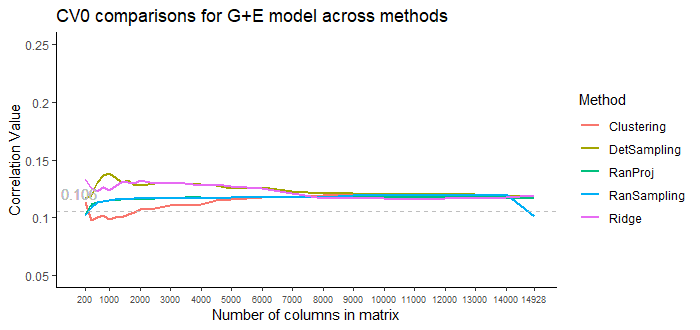
\includegraphics[width=0.9\linewidth]{figures/G+E_CV0_All_Methods.png}
       \label{fig:Ng1} 
    \end{subfigure}
    
    \begin{subfigure}
       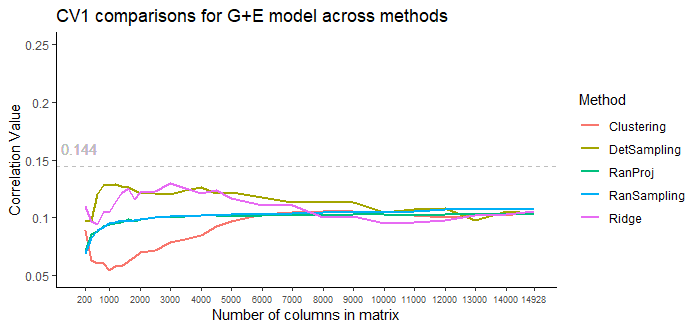
\includegraphics[width=0.9\linewidth]{figures/G+E_CV1_All_Methods.png}
       \label{fig:Ng2}
    \end{subfigure}
    
    \begin{subfigure}
       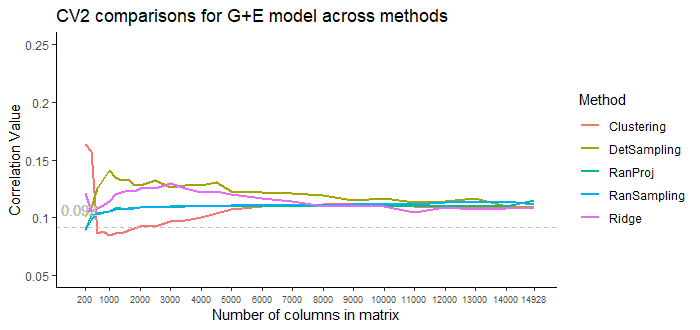
\includegraphics[width=0.9\linewidth]{figures/G+E_CV2_All_Methods.png}
       \label{fig:Ng3}
    \end{subfigure}
\caption{Prediction accuracy of a chickpea population comprising of 306 genotypes tested in 9 environments for the G+E model under the three cross-validation schemes (CV0, CV1, CV2) across 26 different genomic information sizes. \\}
 \label{fig:g_e_all}
\end{figure}

\begin{figure}[H]
\centering
\begin{subfigure}
   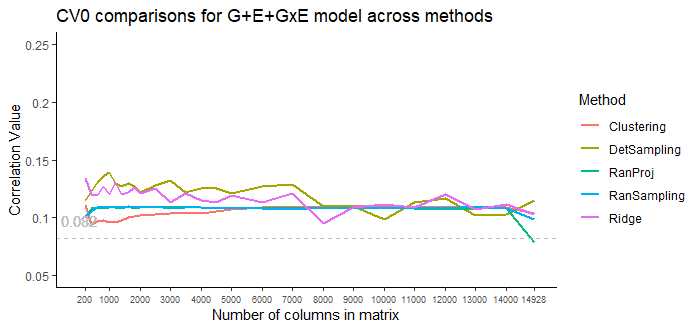
\includegraphics[width=0.9\linewidth]{figures/G+E+GxE_CV0_All_Methods.png}
   \label{fig:Ng4} 
\end{subfigure}

\begin{subfigure}
   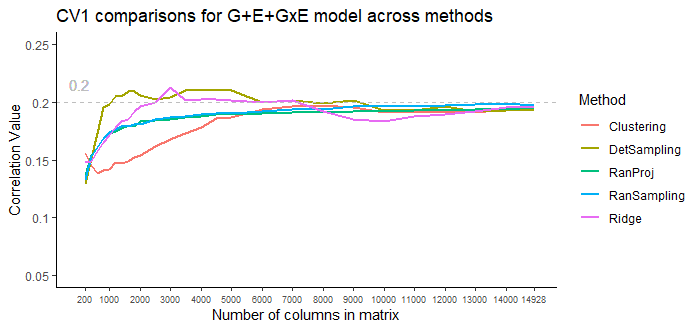
\includegraphics[width=0.9\linewidth]{figures/G+E+GxE_CV1_All_Methods.png}
   \label{fig:Ng5}
\end{subfigure}


\begin{subfigure}
   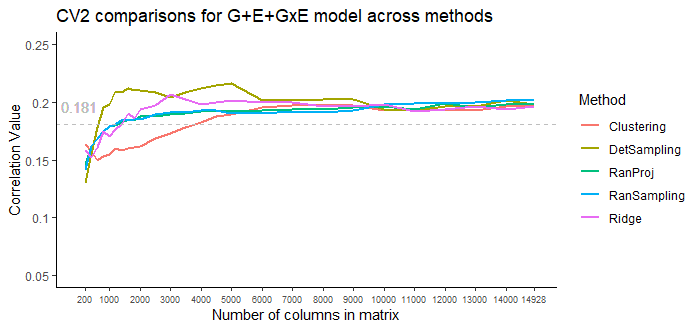
\includegraphics[width=0.9\linewidth]{figures/G+E+GxE_CV2_All_Methods.png}
   \label{fig:Ng6}
\end{subfigure}
\caption{Prediction accuracy of a chickpea population comprising of 306 genotypes tested in 9 environments for the G+E+GxE model under the three cross-validation schemes (CV0, CV1, CV2) across 26 different genomic information sizes. \\}
 \label{fig:gxe_all}
\end{figure}

\section{Results and Discussion}
\label{sec:results}

This study focused on two objectives. The primary objective was to evaluate the merit of using dimensionality reduction methods as a pre-processing step in genomic prediction. We used five dimensionality reduction methods in order to present dimensionality reduction as an effective pre-processing step in genomic prediction and compared their reduction capabilities to find which methods work better for genomic prediction. Second, we studied the trends in prediction accuracy of reduced data sets as a function of their size. \\

To recall, we compared the five dimensionality reduction methods using three genomic prediction models with each model evaluated using three cross-validation schemes. Among the prediction models, the model represented by Eq. \ref{eq:e} is a baseline model with only environmental and line effects. This model does not have genomic effects and hence are not subjected to any dimensionality reduction methods. Thus, the baseline $E+L$ model provides a single prediction accuracy value for each cross-validation scheme. For the other prediction models, each dimensionality reduction method was used to generate reduced marker data sets of 26 different sizes to answer our secondary objective. The results from these models are summarized in the plots in Fig \ref{fig:g_e_all} and Fig \ref{fig:gxe_all}. This chickpea data set was used for genomic prediction in \cite{roorkiwal_genomic-enabled_2018} using the same three genomic prediction models and evaluated with the same three cross-validation schemes. We used their prediction accuracy values as the benchmark to compare our results to. Their paper used the whole genomic data set without any dimensionality reduction and thus served well as a baseline to evaluate dimensionality reduction methods. For each model and cross-validation combination, their results are referenced using a grey horizontal line in the results. The differences in their results and our whole data set results are a consequence of the randomization in the cross-validation folds and hence are not a concern.\\

Irrespective of the model and CV scheme, all dimensionality reduction methods required only a fraction of the total input markers to obtain maximum correlation. In addition, we observed a plateauing of correlation values as the number of markers selected increased for all methods. Thus, the  number of markers required to achieve maximum correlation may be an inappropriate measure to evaluate the reduction capability of the method. Instead, we considered a 95\% of the maximum correlation as our metric to evaluate the reduction methods. For instance, for the CV1 scheme in the G $\times$ E model, the random projection algorithm achieved the maximum correlation of 0.195 with all 14,928 input markers. However, the method achieved a 95\% maximum correlation of 0.185 with just 3000 input markers. This is a significant reduction in the number of input markers for similar correlation values. In fact, for all the dimensionality reduction methods, fewer than 40\% of the input markers were required to achieve a 95\% max correlation value. These results are summarized in Table \ref{tab:cor_max}. Further, for the deterministic sampling and ridge regression based reduction, best correlation was achieved by a reduced data set rather than using the whole data set in all three models indicating the presence of noise in the data. This showed the usefulness of using dimensionality reduction methods as a pre-processing step in genomic prediction to reduce the noise in the data while maintaining or even improving the accuracy of the models. \\

Second, no one reduction method had the best reduction capability across all prediction models and CV combinations. For instance, for the CV2 scheme of the G $\times$ E model, deterministic sampling required only 1200 markers in the input data to achieve 95\% of the maximum correlation compared to 4500 required by clustering. On the other hand, for the CV2 scheme of the G + E model, clustering required only 200 input markers to attain 95\% of the maximum correlation compared to 1000 required by deterministic sampling. Random projection and random sampling methods were very similar to each other in terms of prediction accuracy values across all matrix size by model by cross validation combinations. All of the reduction methods had similar prediction accuracies within the model and CV combination, which reiterates the utility of dimensionality reduction regardless of the method used.



% Please add the following required packages to your document preamble:
% \usepackage{booktabs}
\begin{center}
\begin{table}[]
\centering
\begin{tabular}{@{}lllrr@{}}
\toprule
Pred. model & CV  & DR Method     & \# Cols & Correlation \\ \midrule
G+E+GxE    & CV0 & Clustering  & 200     & 0.105       \\
           &     & DetSampling & 800    & 0.132       \\
           &     & RanProj     & 400    & 0.104        \\
           &     & RanSampling & 400     & 0.104        \\
           &     & Ridge       & 200     & 0.127       \\
           \cline{2-5}
           & CV1 & Clustering  & 4500    & 0.185       \\
           &     & DetSampling & 1200    & 0.199        \\      
           &     & RanProj     & 3000   & 0.185       \\
           &     & RanSampling & 4000   & 0.189       \\       
           &     & Ridge       & 3000    & 0.202       \\ \cline{2-5}
           & CV2 & Clustering  & 4500    & 0.188       \\
           &     & DetSampling & 1200    & 0.205       \\       
           &     & RanProj     & 3000   & 0.189       \\
           &     & RanSampling & 3000   & 0.191       \\
           &     & Ridge       & 2500    & 0.197       \\ \cline{1-5}
G+E        & CV0 & Clustering  & 200    & 0.113       \\
           &     & DetSampling & 600    & 0.131       \\
           &     & RanProj     & 400    & 0.112       \\
           &     & RanSampling & 800   & 0.114        \\
           &     & Ridge       & 200     & 0.126       \\ \cline{2-5}
           & CV1 & Clustering  & 6000    & 0.101       \\
           &     & DetSampling & 800    & 0.123       \\
           &     & RanProj     & 1600    & 0.098       \\
           &     & RanSampling & 5000   & 0.103       \\
           &     & Ridge       & 1600    & 0.124       \\ \cline{2-5}
           & CV2 & Clustering  & 200     & 0.155       \\
           &     & DetSampling & 1000    & 0.134       \\
           &     & RanProj     & 2000   & 0.109       \\
           &     & RanSampling & 1800   & 0.108       \\
           &     & Ridge       & 1600    & 0.124       \\ \cline{1-5}
E+L        & CV0 &             & 14928   & 0.089       \\
           & CV1 &             & 14928   & -0.098      \\
           & CV2 &             & 14928   & 0.045       \\ \bottomrule
\end{tabular}
\caption{Number of markers selected by each dimensionality reduction (DR) method to obtain 95\% of the highest correlation for the three prediction models (G+E+GxE, G+E, E+L) under the three cross-validation schemes (CV0, CV1, CV2).}
\label{tab:cor_max}
\end{table}
\end{center}


\section{Conclusions}
\label{sec:conclusions}

Modern plant breeding programs rely on coupling genomic information with phenotypic performance data to select favorable lines. Early genomic selection models included line, environment, phenotypic and genomic information to predict the performance of lines. Complex traits such as yield are affected by a large number of genomic, environmental factors and their interaction and hence the development of models that allowed for this genotype by environment interactions improved the genomic prediction accuracy. The improvements in genotyping technology combined with the reducing cost has led to the generation of genomic data of enormous sizes which are often high-dimensional in nature. While current genomic selection models are capable of handling these high-dimensional data, there are questions about their efficiency. Further, including information on hundreds of thousands of potentially unrelated markers in the genomic prediction models could negatively impact the prediction accuracy of the trait of interest. Lastly, there is a computational resource cost that must be taken into account. Prediction models with larger input sizes require much greater computational resources to run, both in terms of hardware as well as time. We proposed dimensionality reduction as a mechanism to address all of these concerns.\\

In this study, we used a chickpea data set. Chickpea is the second largest produced food legume crop in the world \cite{roorkiwal_genome-enabled_2016}. It's high protein content makes it a valuable source of protein in several cultures across the world, especially in vegetarian diets. Implementation of GS methods helps breeding programs reduce breeding cycle time and improve the rate of genetic gains \cite{roorkiwal_genomic-enabled_2018} by allowing breeders to select lines using genomic marker data before performing field trials. With the recent improvements in the high-throughput genotyping technologies, millions of markers are available for several hundred lines of chickpea. GS has been adept at accessing these large data sets to predict performance of lines. However, further advances in this area will yield larger marker data sets which could potentially overwhelm the current GS methods as well as the computational resources available. In addition, other high-dimensional data such as high-dimensional weather covariates and high-throughput phenotyping information are increasingly more available in breeding programs. While we did not consider such data in this study, the inclusion of such data could create computational bottlenecks. These reasons present a need for developing methods that effectively handle large data sets and use the additional data available to improve prediction accuracies.  \\

The key contribution of this work was to propose using dimensionality reduction in genomic prediction analyses and show its utility using a handpicked subset of all available methods. For example, we explored the possibility of using randomized algorithms for dimensionality reduction with the help of primitive implementations. There are several more sophisticated randomized algorithms that could improve the dimensionality reduction, which can be explored in future works. Our results act as a proof of concept that future researchers can use to explore various dimensionality reduction methods and identify the best method for their breeding data. Our results clearly indicate the need for integrating dimensionality reduction methods into genomic selection to reduce the computational resource requirements and to improve the prediction process and better select the best performing lines in any breeding program. \\


\section{Acknowledgement}

This research was done using resources provided by the Open Science Grid \cite{osg07, osg09}, which is supported by the National Science Foundation award \#2030508. This work was completed utilizing the Holland Computing Center of the University of Nebraska,
which receives support from the Nebraska Research Initiative. VM was partially supported by the Development of Waxy Sorghum Lines Grant from the Department of Agriculture - NIFA (UNR 19-58). DJ was supported by the Agriculture and Food Research Initiative Grant (NEB-21-176) from the USDA National Institute of Food and Agriculture, Plant Health and Production and Plant Products: Plant Breeding for Agricultural Production, A1211, Accession No. 1015252.
\chapter{Combining Multi-Type Data for High-Dimensional Classification}
    
\section{Introduction}

Most phenotypic traits that have economic and agronomic importance are complex traits that are controlled by multiple genes, each of which have a small effect on the phenotypic expression. The development and subsequent advancements in  high-throughput genotyping technology has enabled the wide-spread use of genomic information for the prediction of phenotypic traits in plant breeding programs. One of the primary objective of plant breeding programs is to cross genotypes that have desirable traits in the hope of increasing genetic gains. The number of genotypes obtained from crosses could be practically infeasible to test on the field. Genomic prediction (GP) allows breeders to efficiently select genotypes that have the best chance of succeeding in field trials. Genomic selection \cite{meuwissen_prediction_2001}, aka genomic prediction, was proposed as a method to use the entire genome to predict the phenotypic traits. The main goal of genomic selection  is to estimate the genomic estimated breeding values (GEBVs) for untested test genotypes with the help of models built using phenotypic and marker information of the training genotypes and use these GEBVs for selection purposes. The testing set contains genomic information for the genotypes, but not their phenotypic information. Since the testing set individuals are not phenotyped, genomic prediction helps reduce the breeding cycle time and consequently saves time, land, and cost. In addition, the ever-reducing cost of genotyping technology has also made genomic prediction methods more attractive for breeding programs.  \\

Several statistical methods have been proposed for GP in the past two decades since \cite{meuwissen_prediction_2001}, which can be categorized into parametric, semi-parametric and non-parametric methods. Some popular parametric methods include Bayes ridge regression, least absolute shrinkage and selection operator (LASSO) \cite{tibshirani1996}, Bayes LASSO \cite{park_casella_2008}, G-BLUP \cite{hayes_accuracy_2009}, BayesA and Bayes B \cite{meuwissen_prediction_2001}. Common semi-parametric and non-parametric methods used in GP are reproducing kernal Hibert spaces (RKHS) \cite{gianola_genomic-assisted_2006, de_los_campos_semi-parametric_2010}, neural networks \cite{gianola_genomic-assisted_2006, gianola_predicting_2011, gonzalez_camacho_2012, perez_rodriguez_2012}, and support vector regression \cite{james_introduction_2013}. Several papers \cite{de_los_campos_2013, heslot_2012, azodi_benchmarking_2019, reka_howard_2014, crain_2018, haroldo_neves_2012, li_zhang_2018} have compared the various prediction methods, and the consensus is that no single method is best performing across all studies. A more comprehensive list of studies comparing the various GP methods can be found here \cite{de_los_campos_2013, montesinos_lopez_2021}. Improvements in computing speed as well as increased availability of graphics processing units (GPUs) has led to rapid improvements in deep learning approaches. Consequently, there is a growing body of literature applying deep learning methods to improve genomic prediction \cite{azodi_benchmarking_2019, montesinos_lopez_2018, montesinos-lopez_new_2019, montesinos_lopez_2021, li_zhang_2018, bellot_2018}. Genomic selection methods have been implemented in crops such as maize \cite{windhausen_2012, perez_rodriguez_2012, crossa_genomic_2014}, wheat \cite{crain_2018, haile_2018, jarquin_increasing_2017}, rice \cite{du_genomic_2018, Xu_rice_2014, spindel2015genomic, zeng2017rational}, legumes \cite{roorkiwal_genome-enabled_2016, roorkiwal_genomic-enabled_2018, burstin2015genetic, varshney2018accelerating}, cassava \cite{okeke2017accuracies, de_oliviera_2012}, apple \cite{roth2020genomic}, etc. \\

Breeders are often interested in categorical phenotypic traits such as resistance to drought or salinity, susceptibility to disease, and days to maturity or flowering. While there is extensive literature covering prediction of continuous traits, there is limited literature developing genomic prediction models for classification. BGLR \cite{perez2014genome} is one of the popular R \cite{Rcite} packages for genomic prediction that implements Bayesian regression models and is capable of handling categorical responses. \cite{ghosal_sparse_2016} proposed a penalized forward selection based support vector classification method for classification in high-dimensional settings and showed superior performance compared to penalized approaches such as LASSO and elastic net as well as classical support vector classification on a genomic data set. \\ 


Modern plant breeding programs are collecting an increasing amount of data of various types and several sources such as multiple secondary phenotypic traits (other than the main trait of interest), high-throughput phenotyping data, weather data, hyper-spectral images, and different types of -omics data such a metabolomics, proteomics, transcriptomics, etc. It is believed that many secondary phenotypic traits are often positively associated with the main trait, a fact that most prediction models do not take advantage of. Given the availability of different data mentioned above, an important question to investigate is how we could integrate these various data types to improve prediction. Early attempts at integration of data types for genomic prediction show promising results \cite{schrag_beyond_2018 , lopez-cruz_regularized_2020, arouisse_improving_2021, sandhu_combining_2021}. \\

Integrating different data types becomes a complex challenge when the data types have very different dimensions. In the case of genomic prediction, the high-dimensional nature of the genomic data is well known. Genomic data is often found to be in the form of Single Nucleotide Polymorphisms (SNPs), which range in the thousands to tens of thousands. On the other hand, data types such as secondary traits are fewer than twenty. Naive concatenation of various data types into existing genomic prediction models could lead to poor results because of the differing sizes. Genomic variables would out-compete all other variable types to explain the variation in the response due to their sheer numbers. A key challenge in such scenarios is to build models that are able to access the unique information present in each data type in order to improve the prediction capabilities. \\

Jarquin et al. (2021; in review) proposed a novel two-step classification method to combine two data types - secondary traits (low-dimensional) and genomic information (high-dimensional). Their method used a penalized forward selection based logistic regression inspired by high-dimensional prediction models such as FIRST \cite{ghosal_first_2009}, STORM \cite{turnbull_iterative_2013}, and penalized forward selection for SVC \cite{ghosal_sparse_2016}. It accounted for the genomic information ``crowding-out" issue and provided sparse models with favorable classification accuracy compared to standard machine learning methods such as random forests, SVMs and FDA. Sparsity in the final models allowed for easier interpretation of relationships between predictors and response, as well as determining important variables. \\

In this chapter, we present an extension to the two-step classification method (Jarquin et al., 2021; in review), where we integrate three data types - secondary traits (low-dimensional), weather (medium-dimensional), and genomic information (high-dimensional). We compared our method to two standard classifiers such as random forests and SVMs. The three-stage method proposed in this work allows us to access the information present in each data type to improve prediction. While the method is developed in an agronomic setting, it can be easily implemented in any application of data-type integration where the data types are of differing dimensions. We believe that the model can be useful in the domain of precision medicine where the main trait can be the susceptibility to disease, the secondary traits being other physiological characteristics of a subject, the medium-dimensional data type being life-style and behavioral characteristics, and the high-dimensional data type being their genomic marker information. \\


The rest of the chapter is organized as follows. First, we present an overview of the method, followed by a detailed description. Next, we describe the data set and its characteristics. Following that, we present the results of the method and compare them to the performance of other standard methods. Finally, we conclude with a discussion and future directions. \\

\section{Overview}

Penalized approaches to regression and classification are common in the presence of high-dimensional data. However, a classical penalized logistic regression approach does not work in our context because it does not allow for variables of certain data types to be considered for model building before others. One of the issues when combining multi-type data when the data are of differing dimensions is that high-dimensional data types such as genomic information outnumber the low-dimensional data types such as secondary traits and subsequently out-compete them to be selected in model building. In a naive concatenation approach, it is plausible that none of the secondary traits or weather variables are retained in the final model. In order to avoid this, we consider a forward selection approach whereby we include variables one at a time. Forward selection also allows control on the order in which data types are considered. By considering low-dimensional data types first, we ensure that all information present that is explaining the variability in the primary trait of interested is used by the classifier, before allowing higher-dimensional data types a chance to explain the variation in the response. \\

Another issue in this problem is that the secondary traits are also impacted by the genomic variables as well as weather variables. Before considering all the variables in the model building, we must remove the effect of genomic and weather variables from the secondary traits and obtain their true intrinsic effects. This also ensures that the potential effect of genomic or weather variables are not mistakenly ascribed to the secondary traits. Separating out the effects will allow for simpler and cleaner interpretation of variable importance and relationships between the response and the explanatory variables. \\

In the first stage of the modeling, we compute the intrinsic effect of the secondary traits devoid of the weather and genomic effects. Let us consider that we have $P$ secondary traits $(U_1, U_2, \dots, U_P)$, $Q$ weather variables $(W_1, W_2, \dots, W_Q)$, and $R$ genomic variables $(V_1, V_2, \dots, V_R)$. In order to remove the genomic and weather effects, we first regress the secondary traits on the set of weather variables, collect the residuals and then regress each of the residuals on the set of genomic variables to obtain double residuals $( \doublehat{U}_{1}, \doublehat{U}_{2}, \dots, \doublehat{U}_{P})$. Since the number of weather variables and genomic variables could be larger than the number of genotypes, least squares regression gives non-unique solutions that may not be stable. Hence, we use penalized regression methods such as adaptive LASSO and ridge regression. Adaptive LASSO \cite{zou2006adaptive} was proposed as an alternative to LASSO in the presence of high multicollinearity among explanatory variables, which is seen commonly in genomic data sets. \\

In the second stage of the modeling, we use a training data set to build a logistic regression classifier in combination with a penalized forward selection scheme to include phenotypic residuals into the model before allowing weather variables and then allowing weather variables before allowing genomic variables. Through the iterative process of the forward selection scheme, we only select the most influential predictor at each step to enter the model. The coefficients of the logistic regression model are obtained through Newton-Raphson updates. \\

Traditionally, a threshold of $p = 0.5$ is used for classification of predicted probabilities from the logistic classifier. However, depending on the class imbalance and the final form of the logistic classifier, this threshold may not be optimal in every scenario. Hence, in the third stage of modeling, we use an optimization data set to determine the optimal threshold to improve classification accuracy. Finally, we use the coefficients from stage 2 and the optimal threshold from stage 3 to predict the class assignment in the test data set and use the results to evaluate the performance of the model. \\

\section{Methods}

Let the binary main trait of interest be represented by $y_i$, the double residual secondary traits be denoted by $\doublehat{u}_i = (\doublehat{u}_{i1}, \doublehat{u}_{i2}, \dots, \doublehat{u}_{iP})$, the weather covariates be denoted by $w_i = (w_{i1}, w_{i2}, \dots, w_{iQ})$, and the genomic variables be denoted by $v_i = (v_{i1}, v_{i2}, \dots, v_{iR})$,  where $i = 1, 2, \dots, n$. Without loss of generality, let us assume that $E(U) = E(W) = E(V) = 0$ and $Var(U) = I_P$, $Var(W) = I_Q$, and $Var(v) = I_R$, where $U = (u_1,  u_2, \dots, u_n)$, $V = (v_1, v_2, \dots, v_n)$, and $W = (w_1, w_2, \dots, w_n)$. This can be implemented by replacing the variables with their standardized versions.  \\

The first stage of the method involves evaluating the double residuals of the secondary traits by removing the effects of weather and genomic covariates. We use a penalized regression model to compute the residuals of each $u_{ip}$, where $p = 1, 2, \dots, P$. First, we  regress each of the secondary traits $u_{ip}$ on the weather variables and obtain the residuals $\hat{u}_{ip} = u_{ip} - w_i^T \hat{b}_p$, where $\hat{b}_p = (\hat{b}_{p1},\hat{b}_{p2}, \dots, \hat{b}_{pQ})$ are the corresponding regression coefficients. The regression coefficients are estimated by minimizing the penalized sum of squares:

\begin{equation}
    \sum_{i= 1}^n (u_{ip} - w_i^T b_p)^2 + \lambda \sum_{q = 1}^Q \text{pen}(|b_{pq}|),
\end{equation}

where the penalty function can be any of the standard penalty functions such as LASSO, aLASSO, ridge regression or SCAD penalties. We compared the various penalty functions, including the raw residuals with zero penalty, to determine which yielded in the best results. Each of the residuals are then regressed on the set of genomic variables through another round of penalized regression implementation to obtain the double residuals $\doublehat{u}_{ip} = \hat{u}_{ip} - v_i^T \hat{d}_p$, where $\hat{d}_p = (\hat{d}_{p1},\hat{d}_{p2}, \dots, \hat{d}_{pR})$ are the corresponding regression coefficients which are obtained by minimizing the following penalized sum of squares:

\begin{equation}
    \sum_{i= 1}^n (\hat{u}_{ip} - v_i^T d_p)^2 + \lambda \sum_{r = 1}^R \text{pen}(|d_{pr}|).
\end{equation}

Here again, the penalty function can take any of the forms mentioned above. \\

After obtaining the intrinsic effect of the secondary traits which are represented by the double residuals obtained in the step one, we move on to the second stage of the method. Here, we implement the penalized forward selection to ensure that the double residuals are entered first into the model, followed by the weather covariates, and then followed by the genomic variables. This ensures that higher-dimensional data types do not overwhelm the smaller-dimensional data types and improve the variability in the response explained by the variables included in the model. We use a logistic classifier as the model structure for its simplicity and ease of interpretability. The probability mass function (PMF) of the $C$-class multinomial logistic classifier for class $c$ is given by:

\begin{equation} \label{eq:pmf}
    P(Y_i = c | \Theta) = \frac{\exp{\sum_{p = 1}^P \alpha_{cp} \doublehat{u}_{ip} + \sum_{q = 1}^Q \beta_{cq} w_{iq} + \sum_{r = 1}^R \gamma_{cr} v_{ir} }}{1 + \sum^C_{{c'}= 1} \exp{\sum_{p = 1}^P \alpha_{c'p} \doublehat{u}_{ip} + \sum_{q = 1}^Q \beta_{c'q} w_{iq} + \sum_{r = 1}^R \gamma_{c'r} v_{ir} } }, 
\end{equation}

where $\Theta = (\alpha_{c1}, \alpha_{c2}, \dots, \alpha_{cP}, \beta_{c1}, \beta_{c2}, \dots, \beta_{cQ}, \gamma_{c1}, \gamma_{c2}, \dots, \gamma_{cR})$ is a $C \times T$ matrix where $T = P + Q + R$. The classification for a new test observation is given by:
\begin{equation}
    \hat{c} = \arg \max_c P(Y_{(n+1)} = c | \hat{\Theta}),
\end{equation}

where $\hat{\Theta}$ is the set of coefficient estimates obtained from the Newton-Raphson estimation method with a LASSO penalty. \\

\subsection{Newton-Raphson (NR) Method}

Using the PMF function defined in Eqn. \ref{eq:pmf}, the log-likelihood function required for the NR method is given by:

\begin{equation} \label{eq:log-lik}
\begin{split}
    f(\theta_{ct}|S) & = \sum_{i:y_i = c} \log\left( \frac{\exp{\sum_{p = 1}^P \alpha_{cp} \doublehat{u}_{ip} + \sum_{q = 1}^Q \beta_{cq} w_{iq} + \sum_{r = 1}^R \gamma_{cr} v_{ir} }}{1 + \sum^C_{{c'}= 1} \exp{\sum_{p = 1}^P \alpha_{c'p} \doublehat{u}_{ip} + \sum_{q = 1}^Q \beta_{c'q} w_{iq} + \sum_{r = 1}^R \gamma_{c'r} v_{ir} } } \right) \\
    & +
    \sum_{i:y_i \neq c} \log\left( \frac{\exp{\sum_{p = 1}^P \alpha_{cp} \doublehat{u}_{ip} + \sum_{q = 1}^Q \beta_{cq} w_{iq} + \sum_{r = 1}^R \gamma_{cr} v_{ir} }}{1 + \sum^C_{{c'}= 1} \exp{\sum_{p = 1}^P \alpha_{c'p} \doublehat{u}_{ip} + \sum_{q = 1}^Q \beta_{c'q} w_{iq} + \sum_{r = 1}^R \gamma_{c'r} v_{ir} } } \right),
\end{split}
\end{equation}

where $S = {(y_1, z_1), \dots, (y_n, z_n)}$ denotes the set of observations with $z_i = (z_{i1}, \dots, z_{iT}) = (\doublehat{u}_{i1}, \dots, \doublehat{u}_{iP}, w_{i1}, \dots, w_{iQ},  v_{i1}, \dots, v_{iR})$. In the presence of a penalty terms for the weather and genomic covariate sets, we maximize a modified version of Eqn. \ref{eq:log-lik}:

\begin{equation} \label{eq:pen-log}
    f(\theta_{ct}|S) - \lambda_1 |\beta_{cq}| - \lambda_2 |\gamma_{cr}|.
\end{equation}

Using the second order Taylor series approximation, the coefficients are updated in the $(k+1)$-th NR iteration as follows:

\begin{align} \label{eq:nr-update1}
    \theta_{ct}^{k+1} (L) & = \theta_{ct}^{k} - s \frac{f' \left(\theta_{ct}^{k} \right) + \max(\lambda_1, \lambda_2, 0)}{f''\left(\theta_{ct}^{k}\right)}  \\ \label{eq:nr-update2}
    \theta_{ct}^{k+1} (R) & = \theta_{ct}^{k} - s \frac{f' \left(\theta_{ct}^{k} \right) - \max(\lambda_1, \lambda_2, 0)}{f''\left(\theta_{ct}^{k}\right)}
\end{align}


More specifically, the NR iteration updates for each of the different data types are given by the following equations:

\begin{align*}
\alpha_{cp}^{k+1} & = \alpha_{cp}^{k} - s \frac{f' \left(\theta_{ct}^{k} \right)}{f''\left(\theta_{ct}^{k}\right)} \\
\beta_{cq}^{k+1} (L) & = \beta_{cq}^{k} - s \frac{f' \left(\theta_{ct}^{k} \right) + \lambda_1}{f''\left(\theta_{ct}^{k}\right)}   &   \beta_{cq}^{k+1} (R) & = \beta_{cq}^{k} - s \frac{f' \left(\theta_{ct}^{k} \right) - \lambda_1}{f''\left(\theta_{ct}^{k}\right)}  \\
\gamma_{cr}^{k+1} (L) & = \gamma_{cr}^{k} - s \frac{f' \left(\theta_{ct}^{k} \right) + \lambda_2}{f''\left(\theta_{ct}^{k}\right)}   &   \beta_{cq}^{k+1} (R) & = \beta_{cq}^{k} - s \frac{f' \left(\theta_{ct}^{k} \right) - \lambda_2}{f''\left(\theta_{ct}^{k}\right)}.
\end{align*}

Here, $L$ and $R$ represent the left- and right-derivatives of Eqn. \ref{eq:pen-log} with respect to $\theta_{ct}$. Following the optimization solution provided in (Wu and Hastie 2009), if $\theta_{ct}^{k+1} (L) < 0$, then we set $\theta_{ct}^{k+1}  = \theta_{ct}^{k+1} (L)$ and if $\theta_{ct}^{k+1} (L) > 0$, we set $\theta_{ct}^{k+1}  = \theta_{ct}^{k+1} (R)$. If either $\theta_{ct}^{k+1} (L) = 0$ or $\theta_{ct}^{k+1} (R) = 0$, then we set $\theta_{ct}^{k+1}  = 0$. The iteration process continues until convergence criteria are met. \\

\subsection{Algorithm}

We initialize the algorithm by setting $\theta_{ct} = 0$ for all $c$ and $t$. Suppose we denote the $k$-th penalized log-likelihood from Eqn. \ref{eq:pen-log} as PLL$_m(c, t)$. 
\begin{enumerate}
    \item Update each $\theta_{ct}$  using the NR update rules from Eqns. \ref{eq:nr-update1} and \ref{eq:nr-update2}. Continue iterations until:
    \begin{equation} \label{eq:pll-1}
        |PLL_m(c, t) - PLL_{m+1}(c,t)| \leq \epsilon |PLL_{m+1}(c,t) + 1|, \text{and}
    \end{equation}
    \begin{equation}\label{eq:pll-2}
        PLL_m(c, t) \leq PLL_{m+1}(c,t).
    \end{equation}
    \item The NR updates start with $s = 1$. If the $\theta_{ct}^{m+1}$ does not satisfy Eqns. \ref{eq:pll-1} or \ref{eq:pll-2}, we repeat the procedure using $ s= 1/2, 1/2^2, 1/2^3, \dots, 1/2^10$. If the PLL does not improve with changing $s$, we set $\theta_{ct}^{m+1} = \theta_{ct}^{m}$.
    \item Stop the iteration process when no variable is selected. 
\end{enumerate}

In the proposed algorithm, there are four hyperparameters that need to be tuned - $s, \epsilon,\lambda_1,$ and $\lambda_2$. We start with step size $s=1$ as a reasonable value for the parameter and vary it by halving it succesively until convergence criteria are met. The $\epsilon$ value is set to $10^{-4}$ as default, but it can be varied. We use a cross-validation grid-search to find the optimal values of $\lambda_1$ and $\lambda_2$, testing various combinations of $\lambda_1$ and $\lambda_2$ ranging from 1 to 10. \\ 

\section{Data}

\section{Results and Discussions}

\section{Conclusion}


%% backmatter is needed at the end of the main body of your thesis to
%% set up page numbering correctly for the remainder of the thesis
\backmatter

%% Start the correct formatting for the appendices
\appendix
%% Input each appendix here
\chapter{Your First Appendix}
    Your appendix text


%% Bibliography goes here (You better have one)
%% BibTeX is your friend

% \bibliographystyle{alpha}  % or use  abbrv to abbreviate first names and use numerical indices
\bibliographystyle{abbrv}  % or use  abbrv to abbreviate first names and use numerical indices
%% Add your BibTex file here (don't include the .bib)
\bibliography{./Chickpea_GenPred_Chapter}



%% Index go here (if you have one)
\end{document}

\endinput
